\documentclass[twoside]{book}

% Packages required by doxygen
\usepackage{fixltx2e}
\usepackage{calc}
\usepackage{doxygen}
\usepackage[export]{adjustbox} % also loads graphicx
\usepackage{graphicx}
\usepackage[utf8]{inputenc}
\usepackage{makeidx}
\usepackage{multicol}
\usepackage{multirow}
\PassOptionsToPackage{warn}{textcomp}
\usepackage{textcomp}
\usepackage[nointegrals]{wasysym}
\usepackage[table]{xcolor}

% Font selection
\usepackage[T1]{fontenc}
\usepackage[scaled=.90]{helvet}
\usepackage{courier}
\usepackage{amssymb}
\usepackage{sectsty}
\renewcommand{\familydefault}{\sfdefault}
\allsectionsfont{%
  \fontseries{bc}\selectfont%
  \color{darkgray}%
}
\renewcommand{\DoxyLabelFont}{%
  \fontseries{bc}\selectfont%
  \color{darkgray}%
}
\newcommand{\+}{\discretionary{\mbox{\scriptsize$\hookleftarrow$}}{}{}}

% Page & text layout
\usepackage{geometry}
\geometry{%
  a4paper,%
  top=2.5cm,%
  bottom=2.5cm,%
  left=2.5cm,%
  right=2.5cm%
}
\tolerance=750
\hfuzz=15pt
\hbadness=750
\setlength{\emergencystretch}{15pt}
\setlength{\parindent}{0cm}
\setlength{\parskip}{3ex plus 2ex minus 2ex}
\makeatletter
\renewcommand{\paragraph}{%
  \@startsection{paragraph}{4}{0ex}{-1.0ex}{1.0ex}{%
    \normalfont\normalsize\bfseries\SS@parafont%
  }%
}
\renewcommand{\subparagraph}{%
  \@startsection{subparagraph}{5}{0ex}{-1.0ex}{1.0ex}{%
    \normalfont\normalsize\bfseries\SS@subparafont%
  }%
}
\makeatother

% Headers & footers
\usepackage{fancyhdr}
\pagestyle{fancyplain}
\fancyhead[LE]{\fancyplain{}{\bfseries\thepage}}
\fancyhead[CE]{\fancyplain{}{}}
\fancyhead[RE]{\fancyplain{}{\bfseries\leftmark}}
\fancyhead[LO]{\fancyplain{}{\bfseries\rightmark}}
\fancyhead[CO]{\fancyplain{}{}}
\fancyhead[RO]{\fancyplain{}{\bfseries\thepage}}
\fancyfoot[LE]{\fancyplain{}{}}
\fancyfoot[CE]{\fancyplain{}{}}
\fancyfoot[RE]{\fancyplain{}{\bfseries\scriptsize Generated by Doxygen }}
\fancyfoot[LO]{\fancyplain{}{\bfseries\scriptsize Generated by Doxygen }}
\fancyfoot[CO]{\fancyplain{}{}}
\fancyfoot[RO]{\fancyplain{}{}}
\renewcommand{\footrulewidth}{0.4pt}
\renewcommand{\chaptermark}[1]{%
  \markboth{#1}{}%
}
\renewcommand{\sectionmark}[1]{%
  \markright{\thesection\ #1}%
}

% Indices & bibliography
\usepackage{natbib}
\usepackage[titles]{tocloft}
\setcounter{tocdepth}{3}
\setcounter{secnumdepth}{5}
\makeindex

% Hyperlinks (required, but should be loaded last)
\usepackage{ifpdf}
\ifpdf
  \usepackage[pdftex,pagebackref=true]{hyperref}
\else
  \usepackage[ps2pdf,pagebackref=true]{hyperref}
\fi
\hypersetup{%
  colorlinks=true,%
  linkcolor=blue,%
  citecolor=blue,%
  unicode%
}

% Custom commands
\newcommand{\clearemptydoublepage}{%
  \newpage{\pagestyle{empty}\cleardoublepage}%
}

\usepackage{caption}
\captionsetup{labelsep=space,justification=centering,font={bf},singlelinecheck=off,skip=4pt,position=top}

%===== C O N T E N T S =====

\begin{document}

% Titlepage & ToC
\hypersetup{pageanchor=false,
             bookmarksnumbered=true,
             pdfencoding=unicode
            }
\pagenumbering{alph}
\begin{titlepage}
\vspace*{7cm}
\begin{center}%
{\Large A\+R\+C\+\_\+decon \\[1ex]\large 0.\+1 }\\
\vspace*{1cm}
{\large Generated by Doxygen 1.8.15}\\
\end{center}
\end{titlepage}
\clearemptydoublepage
\pagenumbering{roman}
\tableofcontents
\clearemptydoublepage
\pagenumbering{arabic}
\hypersetup{pageanchor=true}

%--- Begin generated contents ---
\chapter{readme}
\label{md_readme}
\Hypertarget{md_readme}
$\sim$$\sim$$\sim$ R\+A\+D\+\_\+\+R\+E\+AD R\+E\+A\+D\+ME $\sim$$\sim$$\sim$

//////////////////////////////////// // // // // // P\+S\+QL -\/ A basic tutorial // // // // // ////////////////////////////////////

Step 1\+: P\+S\+QL install

If on current linux, we can find postgre\+S\+QL on synaptic package manager. Simply search under \char`\"{}name\char`\"{} for \char`\"{}postgresql\char`\"{}. Everything should work out nicely, no dpkg required.

Step 2\+: Creating a database

Open a shell (I like bash). We\textquotesingle{}re gonna change user to root, then change to user \char`\"{}postgres\char`\"{} from there. To accomplish this, we do\+:

sudo su

su -\/ postgres

Now, we can create psql users and databases. For now, we\textquotesingle{}ll stick with user \char`\"{}postgres\char`\"{}. To create a database, we do\+:

createdb -\/O postgres testdb

This creates a database called \char`\"{}testdb\char`\"{} with owner \char`\"{}postgres\char`\"{}.

Now, before we go any further, we have to take a look at the psql network settings. Find the \char`\"{}pg\+\_\+hba.\+conf\char`\"{} file that was installed with psql. By default, it should be located at /etc/postgresql/$<$version-\/number$>$/main/. Open this file, and take a look at the line under the heading \char`\"{}\+I\+Pv4 local
  connections\char`\"{}. Make a note of the IP address, then close the file. This is the local address we will use to make a connection to a local psql database. Usually, this address will be 127.\+0.\+0.\+1.

Step 3\+: Getting into the database

We can now make alterations to our database. But before that, we have to set a password for our new user \char`\"{}postgres\char`\"{}. We can do this in another shell (with the default user). Open a shell, and do\+:

sudo -\/u postgres psql postgres

This will provide access into the psql shell layer. From there, we can do

postgres

By default, no password is set. Set the password to whatever you want, just don\textquotesingle{}t forget it!

Now that we\textquotesingle{}ve done that, go back to the shell in which you have changed to user \char`\"{}postgres\char`\"{}. To get into the database we created above, we can do\+:

psql postgres -\/h $<$I\+P-\/address$>$ -\/d testdb

This will prompt for a password, which you should have now. We operating within the database and can make edits.

Step 4\+: Adding data

Tables are used to hold data within psql databases. To create a table while operating within a table, we can do\+:

create table $<$table-\/name$>$ ( $<$data-\/spec1$>$ $<$data-\/type$>$ $<$data-\/spec2$>$ $<$data-\/type$>$ ... ... )

In this instantiation, the data-\/spec refers to the name of the data column. some examples of this could be \char`\"{}names\char`\"{}, \char`\"{}phonenumbers\char`\"{} or \char`\"{}addresses\char`\"{}. The data-\/type signifies what form the variables within the data columns will take. Examples are \char`\"{}integer\char`\"{}, varchar(20) (which indicates a string of 20 chars or less) and char(10) (which indicates a numeral string of 10 digits or less). 
\chapter{Class Index}
\section{Class List}
Here are the classes, structs, unions and interfaces with brief descriptions\+:\begin{DoxyCompactList}
\item\contentsline{section}{\mbox{\hyperlink{classdata__read}{data\+\_\+read}} }{\pageref{classdata__read}}{}
\item\contentsline{section}{\mbox{\hyperlink{classgold__decon}{gold\+\_\+decon}} }{\pageref{classgold__decon}}{}
\item\contentsline{section}{\mbox{\hyperlink{classhisto}{histo}} }{\pageref{classhisto}}{}
\item\contentsline{section}{\mbox{\hyperlink{classresp__read}{resp\+\_\+read}} }{\pageref{classresp__read}}{}
\item\contentsline{section}{\mbox{\hyperlink{classsim__source}{sim\+\_\+source}} }{\pageref{classsim__source}}{}
\item\contentsline{section}{\mbox{\hyperlink{classspatial__decon}{spatial\+\_\+decon}} }{\pageref{classspatial__decon}}{}
\end{DoxyCompactList}

\chapter{File Index}
\section{File List}
Here is a list of all files with brief descriptions\+:\begin{DoxyCompactList}
\item\contentsline{section}{\mbox{\hyperlink{decon__main_8cc}{decon\+\_\+main.\+cc}} }{\pageref{decon__main_8cc}}{}
\item\contentsline{section}{C\+Make\+Files/\mbox{\hyperlink{feature__tests_8c}{feature\+\_\+tests.\+c}} }{\pageref{feature__tests_8c}}{}
\item\contentsline{section}{C\+Make\+Files/\mbox{\hyperlink{feature__tests_8cxx}{feature\+\_\+tests.\+cxx}} }{\pageref{feature__tests_8cxx}}{}
\item\contentsline{section}{C\+Make\+Files/3.\+9.\+1/\+Compiler\+Id\+C/\mbox{\hyperlink{_c_make_c_compiler_id_8c}{C\+Make\+C\+Compiler\+Id.\+c}} }{\pageref{_c_make_c_compiler_id_8c}}{}
\item\contentsline{section}{C\+Make\+Files/3.\+9.\+1/\+Compiler\+Id\+C\+X\+X/\mbox{\hyperlink{_c_make_c_x_x_compiler_id_8cpp}{C\+Make\+C\+X\+X\+Compiler\+Id.\+cpp}} }{\pageref{_c_make_c_x_x_compiler_id_8cpp}}{}
\item\contentsline{section}{include/\mbox{\hyperlink{data__read_8hh}{data\+\_\+read.\+hh}} }{\pageref{data__read_8hh}}{}
\item\contentsline{section}{include/\mbox{\hyperlink{gold__decon_8hh}{gold\+\_\+decon.\+hh}} }{\pageref{gold__decon_8hh}}{}
\item\contentsline{section}{include/\mbox{\hyperlink{histo_8hh}{histo.\+hh}} }{\pageref{histo_8hh}}{}
\item\contentsline{section}{include/\mbox{\hyperlink{resp__read_8hh}{resp\+\_\+read.\+hh}} }{\pageref{resp__read_8hh}}{}
\item\contentsline{section}{include/\mbox{\hyperlink{sim__source_8hh}{sim\+\_\+source.\+hh}} }{\pageref{sim__source_8hh}}{}
\item\contentsline{section}{include/\mbox{\hyperlink{spatial__decon_8hh}{spatial\+\_\+decon.\+hh}} }{\pageref{spatial__decon_8hh}}{}
\item\contentsline{section}{source\+\_\+sims/\mbox{\hyperlink{source_sim3_8m}{source\+Sim3.\+m}} }{\pageref{source_sim3_8m}}{}
\item\contentsline{section}{src/\mbox{\hyperlink{data__read_8cc}{data\+\_\+read.\+cc}} }{\pageref{data__read_8cc}}{}
\item\contentsline{section}{src/\mbox{\hyperlink{gold__decon_8cc}{gold\+\_\+decon.\+cc}} }{\pageref{gold__decon_8cc}}{}
\item\contentsline{section}{src/\mbox{\hyperlink{histo_8cc}{histo.\+cc}} }{\pageref{histo_8cc}}{}
\item\contentsline{section}{src/\mbox{\hyperlink{resp__read_8cc}{resp\+\_\+read.\+cc}} }{\pageref{resp__read_8cc}}{}
\item\contentsline{section}{src/\mbox{\hyperlink{sim__source_8cc}{sim\+\_\+source.\+cc}} }{\pageref{sim__source_8cc}}{}
\item\contentsline{section}{src/\mbox{\hyperlink{spatial__decon_8cc}{spatial\+\_\+decon.\+cc}} }{\pageref{spatial__decon_8cc}}{}
\item\contentsline{section}{tests/\mbox{\hyperlink{data__read__test_8cc}{data\+\_\+read\+\_\+test.\+cc}} }{\pageref{data__read__test_8cc}}{}
\item\contentsline{section}{tests/\mbox{\hyperlink{sim__source__test_8cc}{sim\+\_\+source\+\_\+test.\+cc}} }{\pageref{sim__source__test_8cc}}{}
\item\contentsline{section}{tests/\mbox{\hyperlink{source__read_8cc}{source\+\_\+read.\+cc}} }{\pageref{source__read_8cc}}{}
\item\contentsline{section}{tests/\mbox{\hyperlink{unfold_8cc}{unfold.\+cc}} }{\pageref{unfold_8cc}}{}
\end{DoxyCompactList}

\chapter{Class Documentation}
\hypertarget{classdata__read}{}\section{data\+\_\+read Class Reference}
\label{classdata__read}\index{data\+\_\+read@{data\+\_\+read}}


{\ttfamily \#include $<$data\+\_\+read.\+hh$>$}

\subsection*{Public Member Functions}
\begin{DoxyCompactItemize}
\item 
\mbox{\hyperlink{classdata__read_a680a0d19f4ce5b8a4f45e9e8558bc576}{data\+\_\+read}} ()
\item 
\mbox{\hyperlink{classdata__read_aa401f5929f546d0e74ee2aea7640732c}{$\sim$data\+\_\+read}} ()
\end{DoxyCompactItemize}


\subsection{Constructor \& Destructor Documentation}
\mbox{\Hypertarget{classdata__read_a680a0d19f4ce5b8a4f45e9e8558bc576}\label{classdata__read_a680a0d19f4ce5b8a4f45e9e8558bc576}} 
\index{data\+\_\+read@{data\+\_\+read}!data\+\_\+read@{data\+\_\+read}}
\index{data\+\_\+read@{data\+\_\+read}!data\+\_\+read@{data\+\_\+read}}
\subsubsection{\texorpdfstring{data\+\_\+read()}{data\_read()}}
{\footnotesize\ttfamily data\+\_\+read\+::data\+\_\+read (\begin{DoxyParamCaption}{ }\end{DoxyParamCaption})}

\mbox{\Hypertarget{classdata__read_aa401f5929f546d0e74ee2aea7640732c}\label{classdata__read_aa401f5929f546d0e74ee2aea7640732c}} 
\index{data\+\_\+read@{data\+\_\+read}!````~data\+\_\+read@{$\sim$data\+\_\+read}}
\index{````~data\+\_\+read@{$\sim$data\+\_\+read}!data\+\_\+read@{data\+\_\+read}}
\subsubsection{\texorpdfstring{$\sim$data\+\_\+read()}{~data\_read()}}
{\footnotesize\ttfamily data\+\_\+read\+::$\sim$data\+\_\+read (\begin{DoxyParamCaption}{ }\end{DoxyParamCaption})}



The documentation for this class was generated from the following files\+:\begin{DoxyCompactItemize}
\item 
include/\mbox{\hyperlink{data__read_8hh}{data\+\_\+read.\+hh}}\item 
src/\mbox{\hyperlink{data__read_8cc}{data\+\_\+read.\+cc}}\end{DoxyCompactItemize}

\hypertarget{classgold__decon}{}\section{gold\+\_\+decon Class Reference}
\label{classgold__decon}\index{gold\+\_\+decon@{gold\+\_\+decon}}


{\ttfamily \#include $<$gold\+\_\+decon.\+hh$>$}

\subsection*{Public Member Functions}
\begin{DoxyCompactItemize}
\item 
\mbox{\hyperlink{classgold__decon_a922e3b6065ca68996e30abd173c3723d}{gold\+\_\+decon}} (float $\ast$$\ast$, float $\ast$, int, int, int, int, double)
\item 
\mbox{\hyperlink{classgold__decon_a093b144182a8c8045c0ebd9eff0b2f96}{$\sim$gold\+\_\+decon}} ()
\end{DoxyCompactItemize}


\subsection{Constructor \& Destructor Documentation}
\mbox{\Hypertarget{classgold__decon_a922e3b6065ca68996e30abd173c3723d}\label{classgold__decon_a922e3b6065ca68996e30abd173c3723d}} 
\index{gold\+\_\+decon@{gold\+\_\+decon}!gold\+\_\+decon@{gold\+\_\+decon}}
\index{gold\+\_\+decon@{gold\+\_\+decon}!gold\+\_\+decon@{gold\+\_\+decon}}
\subsubsection{\texorpdfstring{gold\+\_\+decon()}{gold\_decon()}}
{\footnotesize\ttfamily gold\+\_\+decon\+::gold\+\_\+decon (\begin{DoxyParamCaption}\item[{float $\ast$$\ast$}]{resp\+Matrix,  }\item[{float $\ast$}]{source,  }\item[{int}]{ssizex,  }\item[{int}]{ssizey,  }\item[{int}]{number\+Iterations,  }\item[{int}]{number\+Repetitions,  }\item[{double}]{boost }\end{DoxyParamCaption})}

\mbox{\Hypertarget{classgold__decon_a093b144182a8c8045c0ebd9eff0b2f96}\label{classgold__decon_a093b144182a8c8045c0ebd9eff0b2f96}} 
\index{gold\+\_\+decon@{gold\+\_\+decon}!````~gold\+\_\+decon@{$\sim$gold\+\_\+decon}}
\index{````~gold\+\_\+decon@{$\sim$gold\+\_\+decon}!gold\+\_\+decon@{gold\+\_\+decon}}
\subsubsection{\texorpdfstring{$\sim$gold\+\_\+decon()}{~gold\_decon()}}
{\footnotesize\ttfamily gold\+\_\+decon\+::$\sim$gold\+\_\+decon (\begin{DoxyParamCaption}{ }\end{DoxyParamCaption})}



The documentation for this class was generated from the following files\+:\begin{DoxyCompactItemize}
\item 
include/\mbox{\hyperlink{gold__decon_8hh}{gold\+\_\+decon.\+hh}}\item 
src/\mbox{\hyperlink{gold__decon_8cc}{gold\+\_\+decon.\+cc}}\end{DoxyCompactItemize}

\hypertarget{classhisto}{}\section{histo Class Reference}
\label{classhisto}\index{histo@{histo}}


{\ttfamily \#include $<$histo.\+hh$>$}

\subsection*{Public Member Functions}
\begin{DoxyCompactItemize}
\item 
\mbox{\hyperlink{classhisto_a2a23e00b9fe044d7fcd38f12142e5c8d}{histo}} (float $\ast$, int)
\item 
\mbox{\hyperlink{classhisto_a385c60385f4f8d1c67050facb05ffc98}{$\sim$histo}} ()
\end{DoxyCompactItemize}


\subsection{Constructor \& Destructor Documentation}
\mbox{\Hypertarget{classhisto_a2a23e00b9fe044d7fcd38f12142e5c8d}\label{classhisto_a2a23e00b9fe044d7fcd38f12142e5c8d}} 
\index{histo@{histo}!histo@{histo}}
\index{histo@{histo}!histo@{histo}}
\subsubsection{\texorpdfstring{histo()}{histo()}}
{\footnotesize\ttfamily histo\+::histo (\begin{DoxyParamCaption}\item[{float $\ast$}]{source\+\_\+matrix,  }\item[{int}]{data\+\_\+len }\end{DoxyParamCaption})}

\mbox{\Hypertarget{classhisto_a385c60385f4f8d1c67050facb05ffc98}\label{classhisto_a385c60385f4f8d1c67050facb05ffc98}} 
\index{histo@{histo}!````~histo@{$\sim$histo}}
\index{````~histo@{$\sim$histo}!histo@{histo}}
\subsubsection{\texorpdfstring{$\sim$histo()}{~histo()}}
{\footnotesize\ttfamily histo\+::$\sim$histo (\begin{DoxyParamCaption}{ }\end{DoxyParamCaption})}



The documentation for this class was generated from the following files\+:\begin{DoxyCompactItemize}
\item 
include/\mbox{\hyperlink{histo_8hh}{histo.\+hh}}\item 
src/\mbox{\hyperlink{histo_8cc}{histo.\+cc}}\end{DoxyCompactItemize}

\hypertarget{classresp__read}{}\section{resp\+\_\+read Class Reference}
\label{classresp__read}\index{resp\+\_\+read@{resp\+\_\+read}}


{\ttfamily \#include $<$resp\+\_\+read.\+hh$>$}

\subsection*{Public Member Functions}
\begin{DoxyCompactItemize}
\item 
\mbox{\hyperlink{classresp__read_ac9785de9ad22ff8dbdddbd084fa2754c}{resp\+\_\+read}} ()
\item 
\mbox{\hyperlink{classresp__read_ac135ec4a7eb50623aaf28eda054ea12c}{$\sim$resp\+\_\+read}} ()
\end{DoxyCompactItemize}


\subsection{Constructor \& Destructor Documentation}
\mbox{\Hypertarget{classresp__read_ac9785de9ad22ff8dbdddbd084fa2754c}\label{classresp__read_ac9785de9ad22ff8dbdddbd084fa2754c}} 
\index{resp\+\_\+read@{resp\+\_\+read}!resp\+\_\+read@{resp\+\_\+read}}
\index{resp\+\_\+read@{resp\+\_\+read}!resp\+\_\+read@{resp\+\_\+read}}
\subsubsection{\texorpdfstring{resp\+\_\+read()}{resp\_read()}}
{\footnotesize\ttfamily resp\+\_\+read\+::resp\+\_\+read (\begin{DoxyParamCaption}{ }\end{DoxyParamCaption})}

\mbox{\Hypertarget{classresp__read_ac135ec4a7eb50623aaf28eda054ea12c}\label{classresp__read_ac135ec4a7eb50623aaf28eda054ea12c}} 
\index{resp\+\_\+read@{resp\+\_\+read}!````~resp\+\_\+read@{$\sim$resp\+\_\+read}}
\index{````~resp\+\_\+read@{$\sim$resp\+\_\+read}!resp\+\_\+read@{resp\+\_\+read}}
\subsubsection{\texorpdfstring{$\sim$resp\+\_\+read()}{~resp\_read()}}
{\footnotesize\ttfamily resp\+\_\+read\+::$\sim$resp\+\_\+read (\begin{DoxyParamCaption}{ }\end{DoxyParamCaption})}



The documentation for this class was generated from the following files\+:\begin{DoxyCompactItemize}
\item 
include/\mbox{\hyperlink{resp__read_8hh}{resp\+\_\+read.\+hh}}\item 
src/\mbox{\hyperlink{resp__read_8cc}{resp\+\_\+read.\+cc}}\end{DoxyCompactItemize}

\hypertarget{classsim__source}{}\section{sim\+\_\+source Class Reference}
\label{classsim__source}\index{sim\+\_\+source@{sim\+\_\+source}}


{\ttfamily \#include $<$sim\+\_\+source.\+hh$>$}

\subsection*{Public Member Functions}
\begin{DoxyCompactItemize}
\item 
\mbox{\hyperlink{classsim__source_a4abc46c1dda4adb14e1749875960d676}{sim\+\_\+source}} (float $\ast$, int)
\item 
\mbox{\hyperlink{classsim__source_a797822a44ea214dde3c167d175f7a13c}{$\sim$sim\+\_\+source}} ()
\end{DoxyCompactItemize}


\subsection{Constructor \& Destructor Documentation}
\mbox{\Hypertarget{classsim__source_a4abc46c1dda4adb14e1749875960d676}\label{classsim__source_a4abc46c1dda4adb14e1749875960d676}} 
\index{sim\+\_\+source@{sim\+\_\+source}!sim\+\_\+source@{sim\+\_\+source}}
\index{sim\+\_\+source@{sim\+\_\+source}!sim\+\_\+source@{sim\+\_\+source}}
\subsubsection{\texorpdfstring{sim\+\_\+source()}{sim\_source()}}
{\footnotesize\ttfamily sim\+\_\+source\+::sim\+\_\+source (\begin{DoxyParamCaption}\item[{float $\ast$}]{resp\+\_\+space,  }\item[{int}]{resp\+\_\+space\+\_\+len }\end{DoxyParamCaption})}

\mbox{\Hypertarget{classsim__source_a797822a44ea214dde3c167d175f7a13c}\label{classsim__source_a797822a44ea214dde3c167d175f7a13c}} 
\index{sim\+\_\+source@{sim\+\_\+source}!````~sim\+\_\+source@{$\sim$sim\+\_\+source}}
\index{````~sim\+\_\+source@{$\sim$sim\+\_\+source}!sim\+\_\+source@{sim\+\_\+source}}
\subsubsection{\texorpdfstring{$\sim$sim\+\_\+source()}{~sim\_source()}}
{\footnotesize\ttfamily sim\+\_\+source\+::$\sim$sim\+\_\+source (\begin{DoxyParamCaption}{ }\end{DoxyParamCaption})}



The documentation for this class was generated from the following files\+:\begin{DoxyCompactItemize}
\item 
include/\mbox{\hyperlink{sim__source_8hh}{sim\+\_\+source.\+hh}}\item 
src/\mbox{\hyperlink{sim__source_8cc}{sim\+\_\+source.\+cc}}\item 
tests/\mbox{\hyperlink{sim__source__test_8cc}{sim\+\_\+source\+\_\+test.\+cc}}\end{DoxyCompactItemize}

\hypertarget{classspatial__decon}{}\section{spatial\+\_\+decon Class Reference}
\label{classspatial__decon}\index{spatial\+\_\+decon@{spatial\+\_\+decon}}


{\ttfamily \#include $<$spatial\+\_\+decon.\+hh$>$}

\subsection*{Public Member Functions}
\begin{DoxyCompactItemize}
\item 
\mbox{\hyperlink{classspatial__decon_ac87a8698a9d10c5317aa21450afb0d5e}{spatial\+\_\+decon}} (float $\ast$, int, float $\ast$$\ast$, int, int, int, int, int, int)
\item 
\mbox{\hyperlink{classspatial__decon_afcb56f288ca1a562f1692ffd22b2e0c7}{$\sim$spatial\+\_\+decon}} ()
\end{DoxyCompactItemize}


\subsection{Constructor \& Destructor Documentation}
\mbox{\Hypertarget{classspatial__decon_ac87a8698a9d10c5317aa21450afb0d5e}\label{classspatial__decon_ac87a8698a9d10c5317aa21450afb0d5e}} 
\index{spatial\+\_\+decon@{spatial\+\_\+decon}!spatial\+\_\+decon@{spatial\+\_\+decon}}
\index{spatial\+\_\+decon@{spatial\+\_\+decon}!spatial\+\_\+decon@{spatial\+\_\+decon}}
\subsubsection{\texorpdfstring{spatial\+\_\+decon()}{spatial\_decon()}}
{\footnotesize\ttfamily spatial\+\_\+decon\+::spatial\+\_\+decon (\begin{DoxyParamCaption}\item[{float $\ast$}]{resp\+\_\+space,  }\item[{int}]{resp\+\_\+space\+\_\+len,  }\item[{float $\ast$$\ast$}]{source\+\_\+space,  }\item[{int}]{survsizey,  }\item[{int}]{survsizex,  }\item[{int}]{fine,  }\item[{int}]{iso\+\_\+count,  }\item[{int}]{iter,  }\item[{int}]{future\+\_\+sight }\end{DoxyParamCaption})}

\mbox{\Hypertarget{classspatial__decon_afcb56f288ca1a562f1692ffd22b2e0c7}\label{classspatial__decon_afcb56f288ca1a562f1692ffd22b2e0c7}} 
\index{spatial\+\_\+decon@{spatial\+\_\+decon}!````~spatial\+\_\+decon@{$\sim$spatial\+\_\+decon}}
\index{````~spatial\+\_\+decon@{$\sim$spatial\+\_\+decon}!spatial\+\_\+decon@{spatial\+\_\+decon}}
\subsubsection{\texorpdfstring{$\sim$spatial\+\_\+decon()}{~spatial\_decon()}}
{\footnotesize\ttfamily spatial\+\_\+decon\+::$\sim$spatial\+\_\+decon (\begin{DoxyParamCaption}{ }\end{DoxyParamCaption})}



The documentation for this class was generated from the following files\+:\begin{DoxyCompactItemize}
\item 
include/\mbox{\hyperlink{spatial__decon_8hh}{spatial\+\_\+decon.\+hh}}\item 
src/\mbox{\hyperlink{spatial__decon_8cc}{spatial\+\_\+decon.\+cc}}\end{DoxyCompactItemize}

\chapter{File Documentation}
\hypertarget{_c_make_c_compiler_id_8c}{}\section{C\+Make\+Files/3.9.1/\+Compiler\+Id\+C/\+C\+Make\+C\+Compiler\+Id.c File Reference}
\label{_c_make_c_compiler_id_8c}\index{C\+Make\+Files/3.\+9.\+1/\+Compiler\+Id\+C/\+C\+Make\+C\+Compiler\+Id.\+c@{C\+Make\+Files/3.\+9.\+1/\+Compiler\+Id\+C/\+C\+Make\+C\+Compiler\+Id.\+c}}
\subsection*{Macros}
\begin{DoxyCompactItemize}
\item 
\#define \mbox{\hyperlink{_c_make_c_compiler_id_8c_a81dee0709ded976b2e0319239f72d174}{C\+O\+M\+P\+I\+L\+E\+R\+\_\+\+ID}}~\char`\"{}\char`\"{}
\item 
\#define \mbox{\hyperlink{_c_make_c_compiler_id_8c_a2ae9b72bb13abaabfcf2ee0ba7d3fa1d}{S\+T\+R\+I\+N\+G\+I\+F\+Y\+\_\+\+H\+E\+L\+P\+ER}}(X)~\#X
\item 
\#define \mbox{\hyperlink{_c_make_c_compiler_id_8c_a43e1cad902b6477bec893cb6430bd6c8}{S\+T\+R\+I\+N\+G\+I\+FY}}(X)~\mbox{\hyperlink{_c_make_c_x_x_compiler_id_8cpp_a2ae9b72bb13abaabfcf2ee0ba7d3fa1d}{S\+T\+R\+I\+N\+G\+I\+F\+Y\+\_\+\+H\+E\+L\+P\+ER}}(X)
\item 
\#define \mbox{\hyperlink{_c_make_c_compiler_id_8c_adbc5372f40838899018fadbc89bd588b}{P\+L\+A\+T\+F\+O\+R\+M\+\_\+\+ID}}
\item 
\#define \mbox{\hyperlink{_c_make_c_compiler_id_8c_aba35d0d200deaeb06aee95ca297acb28}{A\+R\+C\+H\+I\+T\+E\+C\+T\+U\+R\+E\+\_\+\+ID}}
\item 
\#define \mbox{\hyperlink{_c_make_c_compiler_id_8c_ad1280362da42492bbc11aa78cbf776ad}{D\+EC}}(\mbox{\hyperlink{source_sim3_8m_afde56a346740bd8c5e1e00304507601d}{n}})
\item 
\#define \mbox{\hyperlink{_c_make_c_compiler_id_8c_a46d5d95daa1bef867bd0179594310ed5}{H\+EX}}(\mbox{\hyperlink{source_sim3_8m_afde56a346740bd8c5e1e00304507601d}{n}})
\item 
\#define \mbox{\hyperlink{_c_make_c_compiler_id_8c_a07f8e5783674099cd7f5110e22a78cdb}{C\+\_\+\+D\+I\+A\+L\+E\+CT}}
\end{DoxyCompactItemize}
\subsection*{Functions}
\begin{DoxyCompactItemize}
\item 
int \mbox{\hyperlink{_c_make_c_compiler_id_8c_a0ddf1224851353fc92bfbff6f499fa97}{main}} (int argc, char $\ast$argv\mbox{[}$\,$\mbox{]})
\end{DoxyCompactItemize}
\subsection*{Variables}
\begin{DoxyCompactItemize}
\item 
char const  $\ast$ \mbox{\hyperlink{_c_make_c_compiler_id_8c_a4b0efeb7a5d59313986b3a0390f050f6}{info\+\_\+compiler}} = \char`\"{}I\+N\+FO\char`\"{} \char`\"{}\+:\char`\"{} \char`\"{}compiler\mbox{[}\char`\"{} C\+O\+M\+P\+I\+L\+E\+R\+\_\+\+ID \char`\"{}\mbox{]}\char`\"{}
\item 
char const  $\ast$ \mbox{\hyperlink{_c_make_c_compiler_id_8c_a2321403dee54ee23f0c2fa849c60f7d4}{info\+\_\+platform}} = \char`\"{}I\+N\+FO\char`\"{} \char`\"{}\+:\char`\"{} \char`\"{}platform\mbox{[}\char`\"{} P\+L\+A\+T\+F\+O\+R\+M\+\_\+\+ID \char`\"{}\mbox{]}\char`\"{}
\item 
char const  $\ast$ \mbox{\hyperlink{_c_make_c_compiler_id_8c_a59647e99d304ed33b15cb284c27ed391}{info\+\_\+arch}} = \char`\"{}I\+N\+FO\char`\"{} \char`\"{}\+:\char`\"{} \char`\"{}arch\mbox{[}\char`\"{} A\+R\+C\+H\+I\+T\+E\+C\+T\+U\+R\+E\+\_\+\+ID \char`\"{}\mbox{]}\char`\"{}
\item 
const char $\ast$ \mbox{\hyperlink{_c_make_c_compiler_id_8c_a1ce162bad2fe6966ac8b33cc19e120b8}{info\+\_\+language\+\_\+dialect\+\_\+default}}
\end{DoxyCompactItemize}


\subsection{Macro Definition Documentation}
\mbox{\Hypertarget{_c_make_c_compiler_id_8c_aba35d0d200deaeb06aee95ca297acb28}\label{_c_make_c_compiler_id_8c_aba35d0d200deaeb06aee95ca297acb28}} 
\index{C\+Make\+C\+Compiler\+Id.\+c@{C\+Make\+C\+Compiler\+Id.\+c}!A\+R\+C\+H\+I\+T\+E\+C\+T\+U\+R\+E\+\_\+\+ID@{A\+R\+C\+H\+I\+T\+E\+C\+T\+U\+R\+E\+\_\+\+ID}}
\index{A\+R\+C\+H\+I\+T\+E\+C\+T\+U\+R\+E\+\_\+\+ID@{A\+R\+C\+H\+I\+T\+E\+C\+T\+U\+R\+E\+\_\+\+ID}!C\+Make\+C\+Compiler\+Id.\+c@{C\+Make\+C\+Compiler\+Id.\+c}}
\subsubsection{\texorpdfstring{A\+R\+C\+H\+I\+T\+E\+C\+T\+U\+R\+E\+\_\+\+ID}{ARCHITECTURE\_ID}}
{\footnotesize\ttfamily \#define A\+R\+C\+H\+I\+T\+E\+C\+T\+U\+R\+E\+\_\+\+ID}

\mbox{\Hypertarget{_c_make_c_compiler_id_8c_a07f8e5783674099cd7f5110e22a78cdb}\label{_c_make_c_compiler_id_8c_a07f8e5783674099cd7f5110e22a78cdb}} 
\index{C\+Make\+C\+Compiler\+Id.\+c@{C\+Make\+C\+Compiler\+Id.\+c}!C\+\_\+\+D\+I\+A\+L\+E\+CT@{C\+\_\+\+D\+I\+A\+L\+E\+CT}}
\index{C\+\_\+\+D\+I\+A\+L\+E\+CT@{C\+\_\+\+D\+I\+A\+L\+E\+CT}!C\+Make\+C\+Compiler\+Id.\+c@{C\+Make\+C\+Compiler\+Id.\+c}}
\subsubsection{\texorpdfstring{C\+\_\+\+D\+I\+A\+L\+E\+CT}{C\_DIALECT}}
{\footnotesize\ttfamily \#define C\+\_\+\+D\+I\+A\+L\+E\+CT}

\mbox{\Hypertarget{_c_make_c_compiler_id_8c_a81dee0709ded976b2e0319239f72d174}\label{_c_make_c_compiler_id_8c_a81dee0709ded976b2e0319239f72d174}} 
\index{C\+Make\+C\+Compiler\+Id.\+c@{C\+Make\+C\+Compiler\+Id.\+c}!C\+O\+M\+P\+I\+L\+E\+R\+\_\+\+ID@{C\+O\+M\+P\+I\+L\+E\+R\+\_\+\+ID}}
\index{C\+O\+M\+P\+I\+L\+E\+R\+\_\+\+ID@{C\+O\+M\+P\+I\+L\+E\+R\+\_\+\+ID}!C\+Make\+C\+Compiler\+Id.\+c@{C\+Make\+C\+Compiler\+Id.\+c}}
\subsubsection{\texorpdfstring{C\+O\+M\+P\+I\+L\+E\+R\+\_\+\+ID}{COMPILER\_ID}}
{\footnotesize\ttfamily \#define C\+O\+M\+P\+I\+L\+E\+R\+\_\+\+ID~\char`\"{}\char`\"{}}

\mbox{\Hypertarget{_c_make_c_compiler_id_8c_ad1280362da42492bbc11aa78cbf776ad}\label{_c_make_c_compiler_id_8c_ad1280362da42492bbc11aa78cbf776ad}} 
\index{C\+Make\+C\+Compiler\+Id.\+c@{C\+Make\+C\+Compiler\+Id.\+c}!D\+EC@{D\+EC}}
\index{D\+EC@{D\+EC}!C\+Make\+C\+Compiler\+Id.\+c@{C\+Make\+C\+Compiler\+Id.\+c}}
\subsubsection{\texorpdfstring{D\+EC}{DEC}}
{\footnotesize\ttfamily \#define D\+EC(\begin{DoxyParamCaption}\item[{}]{\mbox{\hyperlink{source_sim3_8m_afde56a346740bd8c5e1e00304507601d}{n}} }\end{DoxyParamCaption})}

{\bfseries Value\+:}
\begin{DoxyCode}
(\textcolor{charliteral}{'0'} + (((\mbox{\hyperlink{source_sim3_8m_afde56a346740bd8c5e1e00304507601d}{n}}) / 10000000)\%10)), \(\backslash\)
  (\textcolor{charliteral}{'0'} + (((\mbox{\hyperlink{source_sim3_8m_afde56a346740bd8c5e1e00304507601d}{n}}) / 1000000)\%10)),  \(\backslash\)
  (\textcolor{charliteral}{'0'} + (((\mbox{\hyperlink{source_sim3_8m_afde56a346740bd8c5e1e00304507601d}{n}}) / 100000)\%10)),   \(\backslash\)
  (\textcolor{charliteral}{'0'} + (((\mbox{\hyperlink{source_sim3_8m_afde56a346740bd8c5e1e00304507601d}{n}}) / 10000)\%10)),    \(\backslash\)
  (\textcolor{charliteral}{'0'} + (((\mbox{\hyperlink{source_sim3_8m_afde56a346740bd8c5e1e00304507601d}{n}}) / 1000)\%10)),     \(\backslash\)
  (\textcolor{charliteral}{'0'} + (((\mbox{\hyperlink{source_sim3_8m_afde56a346740bd8c5e1e00304507601d}{n}}) / 100)\%10)),      \(\backslash\)
  (\textcolor{charliteral}{'0'} + (((\mbox{\hyperlink{source_sim3_8m_afde56a346740bd8c5e1e00304507601d}{n}}) / 10)\%10)),       \(\backslash\)
  (\textcolor{charliteral}{'0'} +  ((\mbox{\hyperlink{source_sim3_8m_afde56a346740bd8c5e1e00304507601d}{n}}) \% 10))
\end{DoxyCode}
\mbox{\Hypertarget{_c_make_c_compiler_id_8c_a46d5d95daa1bef867bd0179594310ed5}\label{_c_make_c_compiler_id_8c_a46d5d95daa1bef867bd0179594310ed5}} 
\index{C\+Make\+C\+Compiler\+Id.\+c@{C\+Make\+C\+Compiler\+Id.\+c}!H\+EX@{H\+EX}}
\index{H\+EX@{H\+EX}!C\+Make\+C\+Compiler\+Id.\+c@{C\+Make\+C\+Compiler\+Id.\+c}}
\subsubsection{\texorpdfstring{H\+EX}{HEX}}
{\footnotesize\ttfamily \#define H\+EX(\begin{DoxyParamCaption}\item[{}]{\mbox{\hyperlink{source_sim3_8m_afde56a346740bd8c5e1e00304507601d}{n}} }\end{DoxyParamCaption})}

{\bfseries Value\+:}
\begin{DoxyCode}
(\textcolor{charliteral}{'0'} + ((\mbox{\hyperlink{source_sim3_8m_afde56a346740bd8c5e1e00304507601d}{n}})>>28 \& 0xF)), \(\backslash\)
  (\textcolor{charliteral}{'0'} + ((\mbox{\hyperlink{source_sim3_8m_afde56a346740bd8c5e1e00304507601d}{n}})>>24 \& 0xF)), \(\backslash\)
  (\textcolor{charliteral}{'0'} + ((\mbox{\hyperlink{source_sim3_8m_afde56a346740bd8c5e1e00304507601d}{n}})>>20 \& 0xF)), \(\backslash\)
  (\textcolor{charliteral}{'0'} + ((\mbox{\hyperlink{source_sim3_8m_afde56a346740bd8c5e1e00304507601d}{n}})>>16 \& 0xF)), \(\backslash\)
  (\textcolor{charliteral}{'0'} + ((\mbox{\hyperlink{source_sim3_8m_afde56a346740bd8c5e1e00304507601d}{n}})>>12 \& 0xF)), \(\backslash\)
  (\textcolor{charliteral}{'0'} + ((\mbox{\hyperlink{source_sim3_8m_afde56a346740bd8c5e1e00304507601d}{n}})>>8  \& 0xF)), \(\backslash\)
  (\textcolor{charliteral}{'0'} + ((\mbox{\hyperlink{source_sim3_8m_afde56a346740bd8c5e1e00304507601d}{n}})>>4  \& 0xF)), \(\backslash\)
  (\textcolor{charliteral}{'0'} + ((\mbox{\hyperlink{source_sim3_8m_afde56a346740bd8c5e1e00304507601d}{n}})     \& 0xF))
\end{DoxyCode}
\mbox{\Hypertarget{_c_make_c_compiler_id_8c_adbc5372f40838899018fadbc89bd588b}\label{_c_make_c_compiler_id_8c_adbc5372f40838899018fadbc89bd588b}} 
\index{C\+Make\+C\+Compiler\+Id.\+c@{C\+Make\+C\+Compiler\+Id.\+c}!P\+L\+A\+T\+F\+O\+R\+M\+\_\+\+ID@{P\+L\+A\+T\+F\+O\+R\+M\+\_\+\+ID}}
\index{P\+L\+A\+T\+F\+O\+R\+M\+\_\+\+ID@{P\+L\+A\+T\+F\+O\+R\+M\+\_\+\+ID}!C\+Make\+C\+Compiler\+Id.\+c@{C\+Make\+C\+Compiler\+Id.\+c}}
\subsubsection{\texorpdfstring{P\+L\+A\+T\+F\+O\+R\+M\+\_\+\+ID}{PLATFORM\_ID}}
{\footnotesize\ttfamily \#define P\+L\+A\+T\+F\+O\+R\+M\+\_\+\+ID}

\mbox{\Hypertarget{_c_make_c_compiler_id_8c_a43e1cad902b6477bec893cb6430bd6c8}\label{_c_make_c_compiler_id_8c_a43e1cad902b6477bec893cb6430bd6c8}} 
\index{C\+Make\+C\+Compiler\+Id.\+c@{C\+Make\+C\+Compiler\+Id.\+c}!S\+T\+R\+I\+N\+G\+I\+FY@{S\+T\+R\+I\+N\+G\+I\+FY}}
\index{S\+T\+R\+I\+N\+G\+I\+FY@{S\+T\+R\+I\+N\+G\+I\+FY}!C\+Make\+C\+Compiler\+Id.\+c@{C\+Make\+C\+Compiler\+Id.\+c}}
\subsubsection{\texorpdfstring{S\+T\+R\+I\+N\+G\+I\+FY}{STRINGIFY}}
{\footnotesize\ttfamily \#define S\+T\+R\+I\+N\+G\+I\+FY(\begin{DoxyParamCaption}\item[{}]{X }\end{DoxyParamCaption})~\mbox{\hyperlink{_c_make_c_x_x_compiler_id_8cpp_a2ae9b72bb13abaabfcf2ee0ba7d3fa1d}{S\+T\+R\+I\+N\+G\+I\+F\+Y\+\_\+\+H\+E\+L\+P\+ER}}(X)}

\mbox{\Hypertarget{_c_make_c_compiler_id_8c_a2ae9b72bb13abaabfcf2ee0ba7d3fa1d}\label{_c_make_c_compiler_id_8c_a2ae9b72bb13abaabfcf2ee0ba7d3fa1d}} 
\index{C\+Make\+C\+Compiler\+Id.\+c@{C\+Make\+C\+Compiler\+Id.\+c}!S\+T\+R\+I\+N\+G\+I\+F\+Y\+\_\+\+H\+E\+L\+P\+ER@{S\+T\+R\+I\+N\+G\+I\+F\+Y\+\_\+\+H\+E\+L\+P\+ER}}
\index{S\+T\+R\+I\+N\+G\+I\+F\+Y\+\_\+\+H\+E\+L\+P\+ER@{S\+T\+R\+I\+N\+G\+I\+F\+Y\+\_\+\+H\+E\+L\+P\+ER}!C\+Make\+C\+Compiler\+Id.\+c@{C\+Make\+C\+Compiler\+Id.\+c}}
\subsubsection{\texorpdfstring{S\+T\+R\+I\+N\+G\+I\+F\+Y\+\_\+\+H\+E\+L\+P\+ER}{STRINGIFY\_HELPER}}
{\footnotesize\ttfamily \#define S\+T\+R\+I\+N\+G\+I\+F\+Y\+\_\+\+H\+E\+L\+P\+ER(\begin{DoxyParamCaption}\item[{}]{X }\end{DoxyParamCaption})~\#X}



\subsection{Function Documentation}
\mbox{\Hypertarget{_c_make_c_compiler_id_8c_a0ddf1224851353fc92bfbff6f499fa97}\label{_c_make_c_compiler_id_8c_a0ddf1224851353fc92bfbff6f499fa97}} 
\index{C\+Make\+C\+Compiler\+Id.\+c@{C\+Make\+C\+Compiler\+Id.\+c}!main@{main}}
\index{main@{main}!C\+Make\+C\+Compiler\+Id.\+c@{C\+Make\+C\+Compiler\+Id.\+c}}
\subsubsection{\texorpdfstring{main()}{main()}}
{\footnotesize\ttfamily int main (\begin{DoxyParamCaption}\item[{int}]{argc,  }\item[{char $\ast$}]{argv\mbox{[}$\,$\mbox{]} }\end{DoxyParamCaption})}



\subsection{Variable Documentation}
\mbox{\Hypertarget{_c_make_c_compiler_id_8c_a59647e99d304ed33b15cb284c27ed391}\label{_c_make_c_compiler_id_8c_a59647e99d304ed33b15cb284c27ed391}} 
\index{C\+Make\+C\+Compiler\+Id.\+c@{C\+Make\+C\+Compiler\+Id.\+c}!info\+\_\+arch@{info\+\_\+arch}}
\index{info\+\_\+arch@{info\+\_\+arch}!C\+Make\+C\+Compiler\+Id.\+c@{C\+Make\+C\+Compiler\+Id.\+c}}
\subsubsection{\texorpdfstring{info\+\_\+arch}{info\_arch}}
{\footnotesize\ttfamily char const$\ast$ info\+\_\+arch = \char`\"{}I\+N\+FO\char`\"{} \char`\"{}\+:\char`\"{} \char`\"{}arch\mbox{[}\char`\"{} A\+R\+C\+H\+I\+T\+E\+C\+T\+U\+R\+E\+\_\+\+ID \char`\"{}\mbox{]}\char`\"{}}

\mbox{\Hypertarget{_c_make_c_compiler_id_8c_a4b0efeb7a5d59313986b3a0390f050f6}\label{_c_make_c_compiler_id_8c_a4b0efeb7a5d59313986b3a0390f050f6}} 
\index{C\+Make\+C\+Compiler\+Id.\+c@{C\+Make\+C\+Compiler\+Id.\+c}!info\+\_\+compiler@{info\+\_\+compiler}}
\index{info\+\_\+compiler@{info\+\_\+compiler}!C\+Make\+C\+Compiler\+Id.\+c@{C\+Make\+C\+Compiler\+Id.\+c}}
\subsubsection{\texorpdfstring{info\+\_\+compiler}{info\_compiler}}
{\footnotesize\ttfamily char const$\ast$ info\+\_\+compiler = \char`\"{}I\+N\+FO\char`\"{} \char`\"{}\+:\char`\"{} \char`\"{}compiler\mbox{[}\char`\"{} C\+O\+M\+P\+I\+L\+E\+R\+\_\+\+ID \char`\"{}\mbox{]}\char`\"{}}

\mbox{\Hypertarget{_c_make_c_compiler_id_8c_a1ce162bad2fe6966ac8b33cc19e120b8}\label{_c_make_c_compiler_id_8c_a1ce162bad2fe6966ac8b33cc19e120b8}} 
\index{C\+Make\+C\+Compiler\+Id.\+c@{C\+Make\+C\+Compiler\+Id.\+c}!info\+\_\+language\+\_\+dialect\+\_\+default@{info\+\_\+language\+\_\+dialect\+\_\+default}}
\index{info\+\_\+language\+\_\+dialect\+\_\+default@{info\+\_\+language\+\_\+dialect\+\_\+default}!C\+Make\+C\+Compiler\+Id.\+c@{C\+Make\+C\+Compiler\+Id.\+c}}
\subsubsection{\texorpdfstring{info\+\_\+language\+\_\+dialect\+\_\+default}{info\_language\_dialect\_default}}
{\footnotesize\ttfamily const char$\ast$ info\+\_\+language\+\_\+dialect\+\_\+default}

{\bfseries Initial value\+:}
\begin{DoxyCode}
=
  \textcolor{stringliteral}{"INFO"} \textcolor{stringliteral}{":"} \textcolor{stringliteral}{"dialect\_default["} \mbox{\hyperlink{_c_make_c_compiler_id_8c_a07f8e5783674099cd7f5110e22a78cdb}{C\_DIALECT}} \textcolor{stringliteral}{"]"}
\end{DoxyCode}
\mbox{\Hypertarget{_c_make_c_compiler_id_8c_a2321403dee54ee23f0c2fa849c60f7d4}\label{_c_make_c_compiler_id_8c_a2321403dee54ee23f0c2fa849c60f7d4}} 
\index{C\+Make\+C\+Compiler\+Id.\+c@{C\+Make\+C\+Compiler\+Id.\+c}!info\+\_\+platform@{info\+\_\+platform}}
\index{info\+\_\+platform@{info\+\_\+platform}!C\+Make\+C\+Compiler\+Id.\+c@{C\+Make\+C\+Compiler\+Id.\+c}}
\subsubsection{\texorpdfstring{info\+\_\+platform}{info\_platform}}
{\footnotesize\ttfamily char const$\ast$ info\+\_\+platform = \char`\"{}I\+N\+FO\char`\"{} \char`\"{}\+:\char`\"{} \char`\"{}platform\mbox{[}\char`\"{} P\+L\+A\+T\+F\+O\+R\+M\+\_\+\+ID \char`\"{}\mbox{]}\char`\"{}}


\hypertarget{_c_make_c_x_x_compiler_id_8cpp}{}\section{C\+Make\+Files/3.9.1/\+Compiler\+Id\+C\+X\+X/\+C\+Make\+C\+X\+X\+Compiler\+Id.cpp File Reference}
\label{_c_make_c_x_x_compiler_id_8cpp}\index{C\+Make\+Files/3.\+9.\+1/\+Compiler\+Id\+C\+X\+X/\+C\+Make\+C\+X\+X\+Compiler\+Id.\+cpp@{C\+Make\+Files/3.\+9.\+1/\+Compiler\+Id\+C\+X\+X/\+C\+Make\+C\+X\+X\+Compiler\+Id.\+cpp}}
\subsection*{Macros}
\begin{DoxyCompactItemize}
\item 
\#define \mbox{\hyperlink{_c_make_c_x_x_compiler_id_8cpp_a81dee0709ded976b2e0319239f72d174}{C\+O\+M\+P\+I\+L\+E\+R\+\_\+\+ID}}~\char`\"{}\char`\"{}
\item 
\#define \mbox{\hyperlink{_c_make_c_x_x_compiler_id_8cpp_a2ae9b72bb13abaabfcf2ee0ba7d3fa1d}{S\+T\+R\+I\+N\+G\+I\+F\+Y\+\_\+\+H\+E\+L\+P\+ER}}(X)~\#X
\item 
\#define \mbox{\hyperlink{_c_make_c_x_x_compiler_id_8cpp_a43e1cad902b6477bec893cb6430bd6c8}{S\+T\+R\+I\+N\+G\+I\+FY}}(X)~\mbox{\hyperlink{_c_make_c_x_x_compiler_id_8cpp_a2ae9b72bb13abaabfcf2ee0ba7d3fa1d}{S\+T\+R\+I\+N\+G\+I\+F\+Y\+\_\+\+H\+E\+L\+P\+ER}}(X)
\item 
\#define \mbox{\hyperlink{_c_make_c_x_x_compiler_id_8cpp_adbc5372f40838899018fadbc89bd588b}{P\+L\+A\+T\+F\+O\+R\+M\+\_\+\+ID}}
\item 
\#define \mbox{\hyperlink{_c_make_c_x_x_compiler_id_8cpp_aba35d0d200deaeb06aee95ca297acb28}{A\+R\+C\+H\+I\+T\+E\+C\+T\+U\+R\+E\+\_\+\+ID}}
\item 
\#define \mbox{\hyperlink{_c_make_c_x_x_compiler_id_8cpp_ad1280362da42492bbc11aa78cbf776ad}{D\+EC}}(\mbox{\hyperlink{source_sim3_8m_afde56a346740bd8c5e1e00304507601d}{n}})
\item 
\#define \mbox{\hyperlink{_c_make_c_x_x_compiler_id_8cpp_a46d5d95daa1bef867bd0179594310ed5}{H\+EX}}(\mbox{\hyperlink{source_sim3_8m_afde56a346740bd8c5e1e00304507601d}{n}})
\end{DoxyCompactItemize}
\subsection*{Functions}
\begin{DoxyCompactItemize}
\item 
int \mbox{\hyperlink{_c_make_c_x_x_compiler_id_8cpp_a0ddf1224851353fc92bfbff6f499fa97}{main}} (int argc, char $\ast$argv\mbox{[}$\,$\mbox{]})
\end{DoxyCompactItemize}
\subsection*{Variables}
\begin{DoxyCompactItemize}
\item 
char const  $\ast$ \mbox{\hyperlink{_c_make_c_x_x_compiler_id_8cpp_a4b0efeb7a5d59313986b3a0390f050f6}{info\+\_\+compiler}} = \char`\"{}I\+N\+FO\char`\"{} \char`\"{}\+:\char`\"{} \char`\"{}compiler\mbox{[}\char`\"{} C\+O\+M\+P\+I\+L\+E\+R\+\_\+\+ID \char`\"{}\mbox{]}\char`\"{}
\item 
char const  $\ast$ \mbox{\hyperlink{_c_make_c_x_x_compiler_id_8cpp_a2321403dee54ee23f0c2fa849c60f7d4}{info\+\_\+platform}} = \char`\"{}I\+N\+FO\char`\"{} \char`\"{}\+:\char`\"{} \char`\"{}platform\mbox{[}\char`\"{} P\+L\+A\+T\+F\+O\+R\+M\+\_\+\+ID \char`\"{}\mbox{]}\char`\"{}
\item 
char const  $\ast$ \mbox{\hyperlink{_c_make_c_x_x_compiler_id_8cpp_a59647e99d304ed33b15cb284c27ed391}{info\+\_\+arch}} = \char`\"{}I\+N\+FO\char`\"{} \char`\"{}\+:\char`\"{} \char`\"{}arch\mbox{[}\char`\"{} A\+R\+C\+H\+I\+T\+E\+C\+T\+U\+R\+E\+\_\+\+ID \char`\"{}\mbox{]}\char`\"{}
\item 
const char $\ast$ \mbox{\hyperlink{_c_make_c_x_x_compiler_id_8cpp_a1ce162bad2fe6966ac8b33cc19e120b8}{info\+\_\+language\+\_\+dialect\+\_\+default}}
\end{DoxyCompactItemize}


\subsection{Macro Definition Documentation}
\mbox{\Hypertarget{_c_make_c_x_x_compiler_id_8cpp_aba35d0d200deaeb06aee95ca297acb28}\label{_c_make_c_x_x_compiler_id_8cpp_aba35d0d200deaeb06aee95ca297acb28}} 
\index{C\+Make\+C\+X\+X\+Compiler\+Id.\+cpp@{C\+Make\+C\+X\+X\+Compiler\+Id.\+cpp}!A\+R\+C\+H\+I\+T\+E\+C\+T\+U\+R\+E\+\_\+\+ID@{A\+R\+C\+H\+I\+T\+E\+C\+T\+U\+R\+E\+\_\+\+ID}}
\index{A\+R\+C\+H\+I\+T\+E\+C\+T\+U\+R\+E\+\_\+\+ID@{A\+R\+C\+H\+I\+T\+E\+C\+T\+U\+R\+E\+\_\+\+ID}!C\+Make\+C\+X\+X\+Compiler\+Id.\+cpp@{C\+Make\+C\+X\+X\+Compiler\+Id.\+cpp}}
\subsubsection{\texorpdfstring{A\+R\+C\+H\+I\+T\+E\+C\+T\+U\+R\+E\+\_\+\+ID}{ARCHITECTURE\_ID}}
{\footnotesize\ttfamily \#define A\+R\+C\+H\+I\+T\+E\+C\+T\+U\+R\+E\+\_\+\+ID}

\mbox{\Hypertarget{_c_make_c_x_x_compiler_id_8cpp_a81dee0709ded976b2e0319239f72d174}\label{_c_make_c_x_x_compiler_id_8cpp_a81dee0709ded976b2e0319239f72d174}} 
\index{C\+Make\+C\+X\+X\+Compiler\+Id.\+cpp@{C\+Make\+C\+X\+X\+Compiler\+Id.\+cpp}!C\+O\+M\+P\+I\+L\+E\+R\+\_\+\+ID@{C\+O\+M\+P\+I\+L\+E\+R\+\_\+\+ID}}
\index{C\+O\+M\+P\+I\+L\+E\+R\+\_\+\+ID@{C\+O\+M\+P\+I\+L\+E\+R\+\_\+\+ID}!C\+Make\+C\+X\+X\+Compiler\+Id.\+cpp@{C\+Make\+C\+X\+X\+Compiler\+Id.\+cpp}}
\subsubsection{\texorpdfstring{C\+O\+M\+P\+I\+L\+E\+R\+\_\+\+ID}{COMPILER\_ID}}
{\footnotesize\ttfamily \#define C\+O\+M\+P\+I\+L\+E\+R\+\_\+\+ID~\char`\"{}\char`\"{}}

\mbox{\Hypertarget{_c_make_c_x_x_compiler_id_8cpp_ad1280362da42492bbc11aa78cbf776ad}\label{_c_make_c_x_x_compiler_id_8cpp_ad1280362da42492bbc11aa78cbf776ad}} 
\index{C\+Make\+C\+X\+X\+Compiler\+Id.\+cpp@{C\+Make\+C\+X\+X\+Compiler\+Id.\+cpp}!D\+EC@{D\+EC}}
\index{D\+EC@{D\+EC}!C\+Make\+C\+X\+X\+Compiler\+Id.\+cpp@{C\+Make\+C\+X\+X\+Compiler\+Id.\+cpp}}
\subsubsection{\texorpdfstring{D\+EC}{DEC}}
{\footnotesize\ttfamily \#define D\+EC(\begin{DoxyParamCaption}\item[{}]{\mbox{\hyperlink{source_sim3_8m_afde56a346740bd8c5e1e00304507601d}{n}} }\end{DoxyParamCaption})}

{\bfseries Value\+:}
\begin{DoxyCode}
(\textcolor{charliteral}{'0'} + (((\mbox{\hyperlink{source_sim3_8m_afde56a346740bd8c5e1e00304507601d}{n}}) / 10000000)\%10)), \(\backslash\)
  (\textcolor{charliteral}{'0'} + (((\mbox{\hyperlink{source_sim3_8m_afde56a346740bd8c5e1e00304507601d}{n}}) / 1000000)\%10)),  \(\backslash\)
  (\textcolor{charliteral}{'0'} + (((\mbox{\hyperlink{source_sim3_8m_afde56a346740bd8c5e1e00304507601d}{n}}) / 100000)\%10)),   \(\backslash\)
  (\textcolor{charliteral}{'0'} + (((\mbox{\hyperlink{source_sim3_8m_afde56a346740bd8c5e1e00304507601d}{n}}) / 10000)\%10)),    \(\backslash\)
  (\textcolor{charliteral}{'0'} + (((\mbox{\hyperlink{source_sim3_8m_afde56a346740bd8c5e1e00304507601d}{n}}) / 1000)\%10)),     \(\backslash\)
  (\textcolor{charliteral}{'0'} + (((\mbox{\hyperlink{source_sim3_8m_afde56a346740bd8c5e1e00304507601d}{n}}) / 100)\%10)),      \(\backslash\)
  (\textcolor{charliteral}{'0'} + (((\mbox{\hyperlink{source_sim3_8m_afde56a346740bd8c5e1e00304507601d}{n}}) / 10)\%10)),       \(\backslash\)
  (\textcolor{charliteral}{'0'} +  ((\mbox{\hyperlink{source_sim3_8m_afde56a346740bd8c5e1e00304507601d}{n}}) \% 10))
\end{DoxyCode}
\mbox{\Hypertarget{_c_make_c_x_x_compiler_id_8cpp_a46d5d95daa1bef867bd0179594310ed5}\label{_c_make_c_x_x_compiler_id_8cpp_a46d5d95daa1bef867bd0179594310ed5}} 
\index{C\+Make\+C\+X\+X\+Compiler\+Id.\+cpp@{C\+Make\+C\+X\+X\+Compiler\+Id.\+cpp}!H\+EX@{H\+EX}}
\index{H\+EX@{H\+EX}!C\+Make\+C\+X\+X\+Compiler\+Id.\+cpp@{C\+Make\+C\+X\+X\+Compiler\+Id.\+cpp}}
\subsubsection{\texorpdfstring{H\+EX}{HEX}}
{\footnotesize\ttfamily \#define H\+EX(\begin{DoxyParamCaption}\item[{}]{\mbox{\hyperlink{source_sim3_8m_afde56a346740bd8c5e1e00304507601d}{n}} }\end{DoxyParamCaption})}

{\bfseries Value\+:}
\begin{DoxyCode}
(\textcolor{charliteral}{'0'} + ((\mbox{\hyperlink{source_sim3_8m_afde56a346740bd8c5e1e00304507601d}{n}})>>28 \& 0xF)), \(\backslash\)
  (\textcolor{charliteral}{'0'} + ((\mbox{\hyperlink{source_sim3_8m_afde56a346740bd8c5e1e00304507601d}{n}})>>24 \& 0xF)), \(\backslash\)
  (\textcolor{charliteral}{'0'} + ((\mbox{\hyperlink{source_sim3_8m_afde56a346740bd8c5e1e00304507601d}{n}})>>20 \& 0xF)), \(\backslash\)
  (\textcolor{charliteral}{'0'} + ((\mbox{\hyperlink{source_sim3_8m_afde56a346740bd8c5e1e00304507601d}{n}})>>16 \& 0xF)), \(\backslash\)
  (\textcolor{charliteral}{'0'} + ((\mbox{\hyperlink{source_sim3_8m_afde56a346740bd8c5e1e00304507601d}{n}})>>12 \& 0xF)), \(\backslash\)
  (\textcolor{charliteral}{'0'} + ((\mbox{\hyperlink{source_sim3_8m_afde56a346740bd8c5e1e00304507601d}{n}})>>8  \& 0xF)), \(\backslash\)
  (\textcolor{charliteral}{'0'} + ((\mbox{\hyperlink{source_sim3_8m_afde56a346740bd8c5e1e00304507601d}{n}})>>4  \& 0xF)), \(\backslash\)
  (\textcolor{charliteral}{'0'} + ((\mbox{\hyperlink{source_sim3_8m_afde56a346740bd8c5e1e00304507601d}{n}})     \& 0xF))
\end{DoxyCode}
\mbox{\Hypertarget{_c_make_c_x_x_compiler_id_8cpp_adbc5372f40838899018fadbc89bd588b}\label{_c_make_c_x_x_compiler_id_8cpp_adbc5372f40838899018fadbc89bd588b}} 
\index{C\+Make\+C\+X\+X\+Compiler\+Id.\+cpp@{C\+Make\+C\+X\+X\+Compiler\+Id.\+cpp}!P\+L\+A\+T\+F\+O\+R\+M\+\_\+\+ID@{P\+L\+A\+T\+F\+O\+R\+M\+\_\+\+ID}}
\index{P\+L\+A\+T\+F\+O\+R\+M\+\_\+\+ID@{P\+L\+A\+T\+F\+O\+R\+M\+\_\+\+ID}!C\+Make\+C\+X\+X\+Compiler\+Id.\+cpp@{C\+Make\+C\+X\+X\+Compiler\+Id.\+cpp}}
\subsubsection{\texorpdfstring{P\+L\+A\+T\+F\+O\+R\+M\+\_\+\+ID}{PLATFORM\_ID}}
{\footnotesize\ttfamily \#define P\+L\+A\+T\+F\+O\+R\+M\+\_\+\+ID}

\mbox{\Hypertarget{_c_make_c_x_x_compiler_id_8cpp_a43e1cad902b6477bec893cb6430bd6c8}\label{_c_make_c_x_x_compiler_id_8cpp_a43e1cad902b6477bec893cb6430bd6c8}} 
\index{C\+Make\+C\+X\+X\+Compiler\+Id.\+cpp@{C\+Make\+C\+X\+X\+Compiler\+Id.\+cpp}!S\+T\+R\+I\+N\+G\+I\+FY@{S\+T\+R\+I\+N\+G\+I\+FY}}
\index{S\+T\+R\+I\+N\+G\+I\+FY@{S\+T\+R\+I\+N\+G\+I\+FY}!C\+Make\+C\+X\+X\+Compiler\+Id.\+cpp@{C\+Make\+C\+X\+X\+Compiler\+Id.\+cpp}}
\subsubsection{\texorpdfstring{S\+T\+R\+I\+N\+G\+I\+FY}{STRINGIFY}}
{\footnotesize\ttfamily \#define S\+T\+R\+I\+N\+G\+I\+FY(\begin{DoxyParamCaption}\item[{}]{X }\end{DoxyParamCaption})~\mbox{\hyperlink{_c_make_c_x_x_compiler_id_8cpp_a2ae9b72bb13abaabfcf2ee0ba7d3fa1d}{S\+T\+R\+I\+N\+G\+I\+F\+Y\+\_\+\+H\+E\+L\+P\+ER}}(X)}

\mbox{\Hypertarget{_c_make_c_x_x_compiler_id_8cpp_a2ae9b72bb13abaabfcf2ee0ba7d3fa1d}\label{_c_make_c_x_x_compiler_id_8cpp_a2ae9b72bb13abaabfcf2ee0ba7d3fa1d}} 
\index{C\+Make\+C\+X\+X\+Compiler\+Id.\+cpp@{C\+Make\+C\+X\+X\+Compiler\+Id.\+cpp}!S\+T\+R\+I\+N\+G\+I\+F\+Y\+\_\+\+H\+E\+L\+P\+ER@{S\+T\+R\+I\+N\+G\+I\+F\+Y\+\_\+\+H\+E\+L\+P\+ER}}
\index{S\+T\+R\+I\+N\+G\+I\+F\+Y\+\_\+\+H\+E\+L\+P\+ER@{S\+T\+R\+I\+N\+G\+I\+F\+Y\+\_\+\+H\+E\+L\+P\+ER}!C\+Make\+C\+X\+X\+Compiler\+Id.\+cpp@{C\+Make\+C\+X\+X\+Compiler\+Id.\+cpp}}
\subsubsection{\texorpdfstring{S\+T\+R\+I\+N\+G\+I\+F\+Y\+\_\+\+H\+E\+L\+P\+ER}{STRINGIFY\_HELPER}}
{\footnotesize\ttfamily \#define S\+T\+R\+I\+N\+G\+I\+F\+Y\+\_\+\+H\+E\+L\+P\+ER(\begin{DoxyParamCaption}\item[{}]{X }\end{DoxyParamCaption})~\#X}



\subsection{Function Documentation}
\mbox{\Hypertarget{_c_make_c_x_x_compiler_id_8cpp_a0ddf1224851353fc92bfbff6f499fa97}\label{_c_make_c_x_x_compiler_id_8cpp_a0ddf1224851353fc92bfbff6f499fa97}} 
\index{C\+Make\+C\+X\+X\+Compiler\+Id.\+cpp@{C\+Make\+C\+X\+X\+Compiler\+Id.\+cpp}!main@{main}}
\index{main@{main}!C\+Make\+C\+X\+X\+Compiler\+Id.\+cpp@{C\+Make\+C\+X\+X\+Compiler\+Id.\+cpp}}
\subsubsection{\texorpdfstring{main()}{main()}}
{\footnotesize\ttfamily int main (\begin{DoxyParamCaption}\item[{int}]{argc,  }\item[{char $\ast$}]{argv\mbox{[}$\,$\mbox{]} }\end{DoxyParamCaption})}



\subsection{Variable Documentation}
\mbox{\Hypertarget{_c_make_c_x_x_compiler_id_8cpp_a59647e99d304ed33b15cb284c27ed391}\label{_c_make_c_x_x_compiler_id_8cpp_a59647e99d304ed33b15cb284c27ed391}} 
\index{C\+Make\+C\+X\+X\+Compiler\+Id.\+cpp@{C\+Make\+C\+X\+X\+Compiler\+Id.\+cpp}!info\+\_\+arch@{info\+\_\+arch}}
\index{info\+\_\+arch@{info\+\_\+arch}!C\+Make\+C\+X\+X\+Compiler\+Id.\+cpp@{C\+Make\+C\+X\+X\+Compiler\+Id.\+cpp}}
\subsubsection{\texorpdfstring{info\+\_\+arch}{info\_arch}}
{\footnotesize\ttfamily char const$\ast$ info\+\_\+arch = \char`\"{}I\+N\+FO\char`\"{} \char`\"{}\+:\char`\"{} \char`\"{}arch\mbox{[}\char`\"{} A\+R\+C\+H\+I\+T\+E\+C\+T\+U\+R\+E\+\_\+\+ID \char`\"{}\mbox{]}\char`\"{}}

\mbox{\Hypertarget{_c_make_c_x_x_compiler_id_8cpp_a4b0efeb7a5d59313986b3a0390f050f6}\label{_c_make_c_x_x_compiler_id_8cpp_a4b0efeb7a5d59313986b3a0390f050f6}} 
\index{C\+Make\+C\+X\+X\+Compiler\+Id.\+cpp@{C\+Make\+C\+X\+X\+Compiler\+Id.\+cpp}!info\+\_\+compiler@{info\+\_\+compiler}}
\index{info\+\_\+compiler@{info\+\_\+compiler}!C\+Make\+C\+X\+X\+Compiler\+Id.\+cpp@{C\+Make\+C\+X\+X\+Compiler\+Id.\+cpp}}
\subsubsection{\texorpdfstring{info\+\_\+compiler}{info\_compiler}}
{\footnotesize\ttfamily char const$\ast$ info\+\_\+compiler = \char`\"{}I\+N\+FO\char`\"{} \char`\"{}\+:\char`\"{} \char`\"{}compiler\mbox{[}\char`\"{} C\+O\+M\+P\+I\+L\+E\+R\+\_\+\+ID \char`\"{}\mbox{]}\char`\"{}}

\mbox{\Hypertarget{_c_make_c_x_x_compiler_id_8cpp_a1ce162bad2fe6966ac8b33cc19e120b8}\label{_c_make_c_x_x_compiler_id_8cpp_a1ce162bad2fe6966ac8b33cc19e120b8}} 
\index{C\+Make\+C\+X\+X\+Compiler\+Id.\+cpp@{C\+Make\+C\+X\+X\+Compiler\+Id.\+cpp}!info\+\_\+language\+\_\+dialect\+\_\+default@{info\+\_\+language\+\_\+dialect\+\_\+default}}
\index{info\+\_\+language\+\_\+dialect\+\_\+default@{info\+\_\+language\+\_\+dialect\+\_\+default}!C\+Make\+C\+X\+X\+Compiler\+Id.\+cpp@{C\+Make\+C\+X\+X\+Compiler\+Id.\+cpp}}
\subsubsection{\texorpdfstring{info\+\_\+language\+\_\+dialect\+\_\+default}{info\_language\_dialect\_default}}
{\footnotesize\ttfamily const char$\ast$ info\+\_\+language\+\_\+dialect\+\_\+default}

{\bfseries Initial value\+:}
\begin{DoxyCode}
= \textcolor{stringliteral}{"INFO"} \textcolor{stringliteral}{":"} \textcolor{stringliteral}{"dialect\_default["}







  \textcolor{stringliteral}{"98"}

\textcolor{stringliteral}{"]"}
\end{DoxyCode}
\mbox{\Hypertarget{_c_make_c_x_x_compiler_id_8cpp_a2321403dee54ee23f0c2fa849c60f7d4}\label{_c_make_c_x_x_compiler_id_8cpp_a2321403dee54ee23f0c2fa849c60f7d4}} 
\index{C\+Make\+C\+X\+X\+Compiler\+Id.\+cpp@{C\+Make\+C\+X\+X\+Compiler\+Id.\+cpp}!info\+\_\+platform@{info\+\_\+platform}}
\index{info\+\_\+platform@{info\+\_\+platform}!C\+Make\+C\+X\+X\+Compiler\+Id.\+cpp@{C\+Make\+C\+X\+X\+Compiler\+Id.\+cpp}}
\subsubsection{\texorpdfstring{info\+\_\+platform}{info\_platform}}
{\footnotesize\ttfamily char const$\ast$ info\+\_\+platform = \char`\"{}I\+N\+FO\char`\"{} \char`\"{}\+:\char`\"{} \char`\"{}platform\mbox{[}\char`\"{} P\+L\+A\+T\+F\+O\+R\+M\+\_\+\+ID \char`\"{}\mbox{]}\char`\"{}}


\hypertarget{feature__tests_8c}{}\section{C\+Make\+Files/feature\+\_\+tests.c File Reference}
\label{feature__tests_8c}\index{C\+Make\+Files/feature\+\_\+tests.\+c@{C\+Make\+Files/feature\+\_\+tests.\+c}}
\subsection*{Functions}
\begin{DoxyCompactItemize}
\item 
int \mbox{\hyperlink{feature__tests_8c_a3c04138a5bfe5d72780bb7e82a18e627}{main}} (int argc, char $\ast$$\ast$argv)
\end{DoxyCompactItemize}
\subsection*{Variables}
\begin{DoxyCompactItemize}
\item 
const char \mbox{\hyperlink{feature__tests_8c_a1582568e32f689337602a16bf8a5bff0}{features}} \mbox{[}$\,$\mbox{]}
\end{DoxyCompactItemize}


\subsection{Function Documentation}
\mbox{\Hypertarget{feature__tests_8c_a3c04138a5bfe5d72780bb7e82a18e627}\label{feature__tests_8c_a3c04138a5bfe5d72780bb7e82a18e627}} 
\index{feature\+\_\+tests.\+c@{feature\+\_\+tests.\+c}!main@{main}}
\index{main@{main}!feature\+\_\+tests.\+c@{feature\+\_\+tests.\+c}}
\subsubsection{\texorpdfstring{main()}{main()}}
{\footnotesize\ttfamily int main (\begin{DoxyParamCaption}\item[{int}]{argc,  }\item[{char $\ast$$\ast$}]{argv }\end{DoxyParamCaption})}



\subsection{Variable Documentation}
\mbox{\Hypertarget{feature__tests_8c_a1582568e32f689337602a16bf8a5bff0}\label{feature__tests_8c_a1582568e32f689337602a16bf8a5bff0}} 
\index{feature\+\_\+tests.\+c@{feature\+\_\+tests.\+c}!features@{features}}
\index{features@{features}!feature\+\_\+tests.\+c@{feature\+\_\+tests.\+c}}
\subsubsection{\texorpdfstring{features}{features}}
{\footnotesize\ttfamily const char features\mbox{[}$\,$\mbox{]}}


\hypertarget{feature__tests_8cxx}{}\section{C\+Make\+Files/feature\+\_\+tests.cxx File Reference}
\label{feature__tests_8cxx}\index{C\+Make\+Files/feature\+\_\+tests.\+cxx@{C\+Make\+Files/feature\+\_\+tests.\+cxx}}
\subsection*{Functions}
\begin{DoxyCompactItemize}
\item 
int \mbox{\hyperlink{feature__tests_8cxx_a3c04138a5bfe5d72780bb7e82a18e627}{main}} (int argc, char $\ast$$\ast$argv)
\end{DoxyCompactItemize}
\subsection*{Variables}
\begin{DoxyCompactItemize}
\item 
const char \mbox{\hyperlink{feature__tests_8cxx_a1582568e32f689337602a16bf8a5bff0}{features}} \mbox{[}$\,$\mbox{]}
\end{DoxyCompactItemize}


\subsection{Function Documentation}
\mbox{\Hypertarget{feature__tests_8cxx_a3c04138a5bfe5d72780bb7e82a18e627}\label{feature__tests_8cxx_a3c04138a5bfe5d72780bb7e82a18e627}} 
\index{feature\+\_\+tests.\+cxx@{feature\+\_\+tests.\+cxx}!main@{main}}
\index{main@{main}!feature\+\_\+tests.\+cxx@{feature\+\_\+tests.\+cxx}}
\subsubsection{\texorpdfstring{main()}{main()}}
{\footnotesize\ttfamily int main (\begin{DoxyParamCaption}\item[{int}]{argc,  }\item[{char $\ast$$\ast$}]{argv }\end{DoxyParamCaption})}



\subsection{Variable Documentation}
\mbox{\Hypertarget{feature__tests_8cxx_a1582568e32f689337602a16bf8a5bff0}\label{feature__tests_8cxx_a1582568e32f689337602a16bf8a5bff0}} 
\index{feature\+\_\+tests.\+cxx@{feature\+\_\+tests.\+cxx}!features@{features}}
\index{features@{features}!feature\+\_\+tests.\+cxx@{feature\+\_\+tests.\+cxx}}
\subsubsection{\texorpdfstring{features}{features}}
{\footnotesize\ttfamily const char features\mbox{[}$\,$\mbox{]}}


\hypertarget{decon__main_8cc}{}\section{decon\+\_\+main.\+cc File Reference}
\label{decon__main_8cc}\index{decon\+\_\+main.\+cc@{decon\+\_\+main.\+cc}}
{\ttfamily \#include $<$string$>$}\newline
{\ttfamily \#include $<$iostream$>$}\newline
{\ttfamily \#include $<$iomanip$>$}\newline
{\ttfamily \#include $<$fstream$>$}\newline
{\ttfamily \#include $<$vector$>$}\newline
{\ttfamily \#include $<$ctime$>$}\newline
{\ttfamily \#include $<$cstdio$>$}\newline
{\ttfamily \#include \char`\"{}data\+\_\+read.\+hh\char`\"{}}\newline
{\ttfamily \#include \char`\"{}gold\+\_\+decon.\+hh\char`\"{}}\newline
{\ttfamily \#include \char`\"{}resp\+\_\+read.\+hh\char`\"{}}\newline
{\ttfamily \#include \char`\"{}histo.\+hh\char`\"{}}\newline
{\ttfamily \#include \char`\"{}sim\+\_\+source.\+hh\char`\"{}}\newline
{\ttfamily \#include \char`\"{}spatial\+\_\+decon.\+hh\char`\"{}}\newline
Include dependency graph for decon\+\_\+main.\+cc\+:
\nopagebreak
\begin{figure}[H]
\begin{center}
\leavevmode
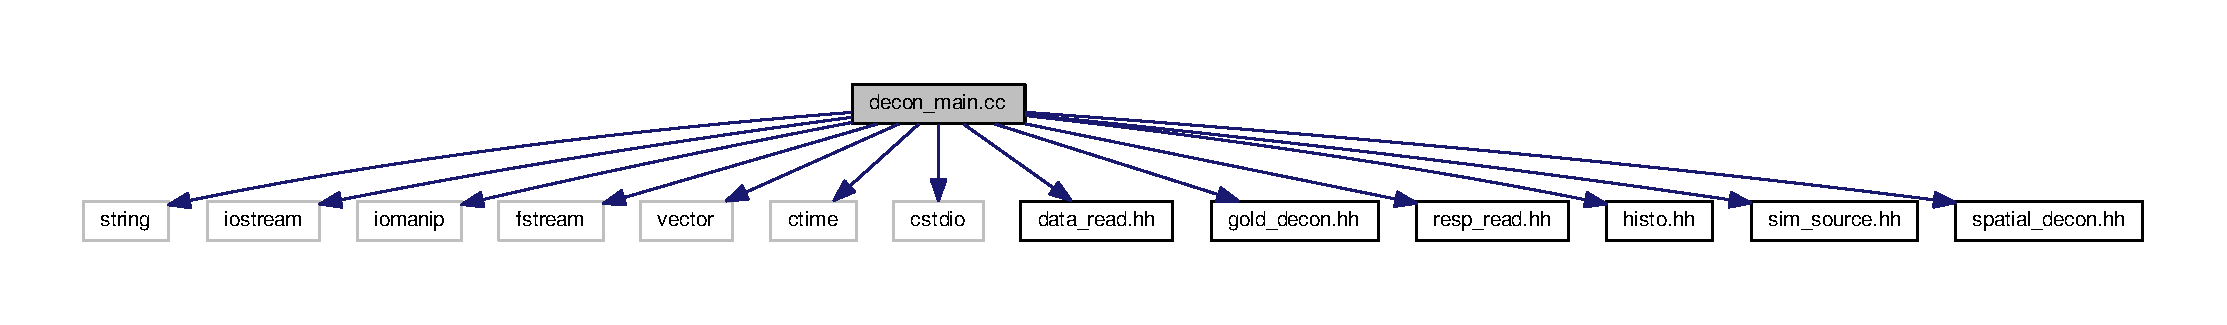
\includegraphics[width=350pt]{decon__main_8cc__incl}
\end{center}
\end{figure}
\subsection*{Functions}
\begin{DoxyCompactItemize}
\item 
int \mbox{\hyperlink{decon__main_8cc_a3c04138a5bfe5d72780bb7e82a18e627}{main}} (int argc, char $\ast$$\ast$argv)
\end{DoxyCompactItemize}
\subsection*{Variables}
\begin{DoxyCompactItemize}
\item 
vector$<$ vector$<$ float $>$ $>$ \mbox{\hyperlink{decon__main_8cc_a9885e2f4f2c1ec5b4d0db16d253892ad}{data\+\_\+mat}}
\item 
int \mbox{\hyperlink{decon__main_8cc_a1adfbfbc200c1f97d6055449f7815076}{data\+\_\+mat\+\_\+len}}
\item 
vector$<$ float $>$ \mbox{\hyperlink{decon__main_8cc_a492d57fd7c64e6f4e02b779824f7c56d}{data\+\_\+sim}}
\item 
vector$<$ vector$<$ float $>$ $>$ \mbox{\hyperlink{decon__main_8cc_a4a66e69e8cc5a880a8ccb008653f1b4c}{space\+\_\+sim}}
\item 
vector$<$ vector$<$ float $>$ $>$ \mbox{\hyperlink{decon__main_8cc_a2904cd77105f4855a21a41efe233992b}{resp\+\_\+mat\+\_\+read}}
\item 
vector$<$ float $>$ \mbox{\hyperlink{decon__main_8cc_a142e4ef7ff0a2b7bf754588286396ca7}{resp\+\_\+space\+\_\+mat\+\_\+read}}
\item 
int \mbox{\hyperlink{decon__main_8cc_aca3c1d36b05c2731d7276b0acc029b3f}{space\+\_\+datax}}
\item 
int \mbox{\hyperlink{decon__main_8cc_a6b37b7991c3851b6fa90ef56decee739}{space\+\_\+datay}}
\item 
vector$<$ vector$<$ int $>$ $>$ \mbox{\hyperlink{decon__main_8cc_a5772281f7b17c2278c30171f82ea8d13}{end\+\_\+ind}}
\item 
float \mbox{\hyperlink{decon__main_8cc_a43cce2495419f8219330c5474b026242}{source\+\_\+decon}} \mbox{[}4096\mbox{]}
\item 
int \mbox{\hyperlink{decon__main_8cc_ab96841bb4729a804d76a68a015d1df14}{iso\+\_\+count}}
\end{DoxyCompactItemize}


\subsection{Function Documentation}
\mbox{\Hypertarget{decon__main_8cc_a3c04138a5bfe5d72780bb7e82a18e627}\label{decon__main_8cc_a3c04138a5bfe5d72780bb7e82a18e627}} 
\index{decon\+\_\+main.\+cc@{decon\+\_\+main.\+cc}!main@{main}}
\index{main@{main}!decon\+\_\+main.\+cc@{decon\+\_\+main.\+cc}}
\subsubsection{\texorpdfstring{main()}{main()}}
{\footnotesize\ttfamily int main (\begin{DoxyParamCaption}\item[{int}]{argc,  }\item[{char $\ast$$\ast$}]{argv }\end{DoxyParamCaption})}



\subsection{Variable Documentation}
\mbox{\Hypertarget{decon__main_8cc_a9885e2f4f2c1ec5b4d0db16d253892ad}\label{decon__main_8cc_a9885e2f4f2c1ec5b4d0db16d253892ad}} 
\index{decon\+\_\+main.\+cc@{decon\+\_\+main.\+cc}!data\+\_\+mat@{data\+\_\+mat}}
\index{data\+\_\+mat@{data\+\_\+mat}!decon\+\_\+main.\+cc@{decon\+\_\+main.\+cc}}
\subsubsection{\texorpdfstring{data\+\_\+mat}{data\_mat}}
{\footnotesize\ttfamily vector$<$ vector$<$float$>$ $>$ data\+\_\+mat}

\mbox{\Hypertarget{decon__main_8cc_a1adfbfbc200c1f97d6055449f7815076}\label{decon__main_8cc_a1adfbfbc200c1f97d6055449f7815076}} 
\index{decon\+\_\+main.\+cc@{decon\+\_\+main.\+cc}!data\+\_\+mat\+\_\+len@{data\+\_\+mat\+\_\+len}}
\index{data\+\_\+mat\+\_\+len@{data\+\_\+mat\+\_\+len}!decon\+\_\+main.\+cc@{decon\+\_\+main.\+cc}}
\subsubsection{\texorpdfstring{data\+\_\+mat\+\_\+len}{data\_mat\_len}}
{\footnotesize\ttfamily int data\+\_\+mat\+\_\+len}

\mbox{\Hypertarget{decon__main_8cc_a492d57fd7c64e6f4e02b779824f7c56d}\label{decon__main_8cc_a492d57fd7c64e6f4e02b779824f7c56d}} 
\index{decon\+\_\+main.\+cc@{decon\+\_\+main.\+cc}!data\+\_\+sim@{data\+\_\+sim}}
\index{data\+\_\+sim@{data\+\_\+sim}!decon\+\_\+main.\+cc@{decon\+\_\+main.\+cc}}
\subsubsection{\texorpdfstring{data\+\_\+sim}{data\_sim}}
{\footnotesize\ttfamily vector$<$float$>$ data\+\_\+sim}

\mbox{\Hypertarget{decon__main_8cc_a5772281f7b17c2278c30171f82ea8d13}\label{decon__main_8cc_a5772281f7b17c2278c30171f82ea8d13}} 
\index{decon\+\_\+main.\+cc@{decon\+\_\+main.\+cc}!end\+\_\+ind@{end\+\_\+ind}}
\index{end\+\_\+ind@{end\+\_\+ind}!decon\+\_\+main.\+cc@{decon\+\_\+main.\+cc}}
\subsubsection{\texorpdfstring{end\+\_\+ind}{end\_ind}}
{\footnotesize\ttfamily vector$<$ vector$<$int$>$ $>$ end\+\_\+ind}

\mbox{\Hypertarget{decon__main_8cc_ab96841bb4729a804d76a68a015d1df14}\label{decon__main_8cc_ab96841bb4729a804d76a68a015d1df14}} 
\index{decon\+\_\+main.\+cc@{decon\+\_\+main.\+cc}!iso\+\_\+count@{iso\+\_\+count}}
\index{iso\+\_\+count@{iso\+\_\+count}!decon\+\_\+main.\+cc@{decon\+\_\+main.\+cc}}
\subsubsection{\texorpdfstring{iso\+\_\+count}{iso\_count}}
{\footnotesize\ttfamily int iso\+\_\+count}

\mbox{\Hypertarget{decon__main_8cc_a2904cd77105f4855a21a41efe233992b}\label{decon__main_8cc_a2904cd77105f4855a21a41efe233992b}} 
\index{decon\+\_\+main.\+cc@{decon\+\_\+main.\+cc}!resp\+\_\+mat\+\_\+read@{resp\+\_\+mat\+\_\+read}}
\index{resp\+\_\+mat\+\_\+read@{resp\+\_\+mat\+\_\+read}!decon\+\_\+main.\+cc@{decon\+\_\+main.\+cc}}
\subsubsection{\texorpdfstring{resp\+\_\+mat\+\_\+read}{resp\_mat\_read}}
{\footnotesize\ttfamily vector$<$ vector$<$float$>$ $>$ resp\+\_\+mat\+\_\+read}

\mbox{\Hypertarget{decon__main_8cc_a142e4ef7ff0a2b7bf754588286396ca7}\label{decon__main_8cc_a142e4ef7ff0a2b7bf754588286396ca7}} 
\index{decon\+\_\+main.\+cc@{decon\+\_\+main.\+cc}!resp\+\_\+space\+\_\+mat\+\_\+read@{resp\+\_\+space\+\_\+mat\+\_\+read}}
\index{resp\+\_\+space\+\_\+mat\+\_\+read@{resp\+\_\+space\+\_\+mat\+\_\+read}!decon\+\_\+main.\+cc@{decon\+\_\+main.\+cc}}
\subsubsection{\texorpdfstring{resp\+\_\+space\+\_\+mat\+\_\+read}{resp\_space\_mat\_read}}
{\footnotesize\ttfamily vector$<$float$>$ resp\+\_\+space\+\_\+mat\+\_\+read}

\mbox{\Hypertarget{decon__main_8cc_a43cce2495419f8219330c5474b026242}\label{decon__main_8cc_a43cce2495419f8219330c5474b026242}} 
\index{decon\+\_\+main.\+cc@{decon\+\_\+main.\+cc}!source\+\_\+decon@{source\+\_\+decon}}
\index{source\+\_\+decon@{source\+\_\+decon}!decon\+\_\+main.\+cc@{decon\+\_\+main.\+cc}}
\subsubsection{\texorpdfstring{source\+\_\+decon}{source\_decon}}
{\footnotesize\ttfamily float source\+\_\+decon\mbox{[}4096\mbox{]}}

\mbox{\Hypertarget{decon__main_8cc_aca3c1d36b05c2731d7276b0acc029b3f}\label{decon__main_8cc_aca3c1d36b05c2731d7276b0acc029b3f}} 
\index{decon\+\_\+main.\+cc@{decon\+\_\+main.\+cc}!space\+\_\+datax@{space\+\_\+datax}}
\index{space\+\_\+datax@{space\+\_\+datax}!decon\+\_\+main.\+cc@{decon\+\_\+main.\+cc}}
\subsubsection{\texorpdfstring{space\+\_\+datax}{space\_datax}}
{\footnotesize\ttfamily int space\+\_\+datax}

\mbox{\Hypertarget{decon__main_8cc_a6b37b7991c3851b6fa90ef56decee739}\label{decon__main_8cc_a6b37b7991c3851b6fa90ef56decee739}} 
\index{decon\+\_\+main.\+cc@{decon\+\_\+main.\+cc}!space\+\_\+datay@{space\+\_\+datay}}
\index{space\+\_\+datay@{space\+\_\+datay}!decon\+\_\+main.\+cc@{decon\+\_\+main.\+cc}}
\subsubsection{\texorpdfstring{space\+\_\+datay}{space\_datay}}
{\footnotesize\ttfamily int space\+\_\+datay}

\mbox{\Hypertarget{decon__main_8cc_a4a66e69e8cc5a880a8ccb008653f1b4c}\label{decon__main_8cc_a4a66e69e8cc5a880a8ccb008653f1b4c}} 
\index{decon\+\_\+main.\+cc@{decon\+\_\+main.\+cc}!space\+\_\+sim@{space\+\_\+sim}}
\index{space\+\_\+sim@{space\+\_\+sim}!decon\+\_\+main.\+cc@{decon\+\_\+main.\+cc}}
\subsubsection{\texorpdfstring{space\+\_\+sim}{space\_sim}}
{\footnotesize\ttfamily vector$<$ vector$<$float$>$ $>$ space\+\_\+sim}


\hypertarget{data__read_8hh}{}\section{include/data\+\_\+read.hh File Reference}
\label{data__read_8hh}\index{include/data\+\_\+read.\+hh@{include/data\+\_\+read.\+hh}}
This graph shows which files directly or indirectly include this file\+:
\nopagebreak
\begin{figure}[H]
\begin{center}
\leavevmode
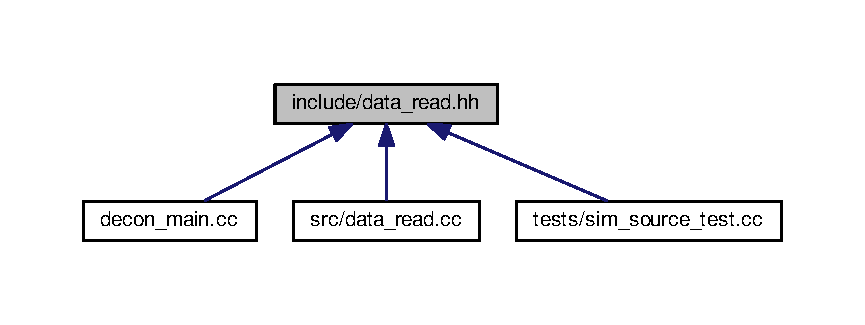
\includegraphics[width=350pt]{data__read_8hh__dep__incl}
\end{center}
\end{figure}
\subsection*{Classes}
\begin{DoxyCompactItemize}
\item 
class \mbox{\hyperlink{classdata__read}{data\+\_\+read}}
\end{DoxyCompactItemize}
\subsection*{Variables}
\begin{DoxyCompactItemize}
\item 
std\+::vector$<$ std\+::vector$<$ float $>$ $>$ \mbox{\hyperlink{data__read_8hh_aa3c8f7c0bda5a845913562e28f9c1818}{data\+\_\+mat}}
\item 
int \mbox{\hyperlink{data__read_8hh_a1adfbfbc200c1f97d6055449f7815076}{data\+\_\+mat\+\_\+len}}
\item 
int \mbox{\hyperlink{data__read_8hh_aca3c1d36b05c2731d7276b0acc029b3f}{space\+\_\+datax}}
\item 
int \mbox{\hyperlink{data__read_8hh_a6b37b7991c3851b6fa90ef56decee739}{space\+\_\+datay}}
\end{DoxyCompactItemize}


\subsection{Variable Documentation}
\mbox{\Hypertarget{data__read_8hh_aa3c8f7c0bda5a845913562e28f9c1818}\label{data__read_8hh_aa3c8f7c0bda5a845913562e28f9c1818}} 
\index{data\+\_\+read.\+hh@{data\+\_\+read.\+hh}!data\+\_\+mat@{data\+\_\+mat}}
\index{data\+\_\+mat@{data\+\_\+mat}!data\+\_\+read.\+hh@{data\+\_\+read.\+hh}}
\subsubsection{\texorpdfstring{data\+\_\+mat}{data\_mat}}
{\footnotesize\ttfamily std\+::vector$<$std\+::vector $<$float$>$ $>$ data\+\_\+mat}

\mbox{\Hypertarget{data__read_8hh_a1adfbfbc200c1f97d6055449f7815076}\label{data__read_8hh_a1adfbfbc200c1f97d6055449f7815076}} 
\index{data\+\_\+read.\+hh@{data\+\_\+read.\+hh}!data\+\_\+mat\+\_\+len@{data\+\_\+mat\+\_\+len}}
\index{data\+\_\+mat\+\_\+len@{data\+\_\+mat\+\_\+len}!data\+\_\+read.\+hh@{data\+\_\+read.\+hh}}
\subsubsection{\texorpdfstring{data\+\_\+mat\+\_\+len}{data\_mat\_len}}
{\footnotesize\ttfamily int data\+\_\+mat\+\_\+len}

\mbox{\Hypertarget{data__read_8hh_aca3c1d36b05c2731d7276b0acc029b3f}\label{data__read_8hh_aca3c1d36b05c2731d7276b0acc029b3f}} 
\index{data\+\_\+read.\+hh@{data\+\_\+read.\+hh}!space\+\_\+datax@{space\+\_\+datax}}
\index{space\+\_\+datax@{space\+\_\+datax}!data\+\_\+read.\+hh@{data\+\_\+read.\+hh}}
\subsubsection{\texorpdfstring{space\+\_\+datax}{space\_datax}}
{\footnotesize\ttfamily int space\+\_\+datax}

\mbox{\Hypertarget{data__read_8hh_a6b37b7991c3851b6fa90ef56decee739}\label{data__read_8hh_a6b37b7991c3851b6fa90ef56decee739}} 
\index{data\+\_\+read.\+hh@{data\+\_\+read.\+hh}!space\+\_\+datay@{space\+\_\+datay}}
\index{space\+\_\+datay@{space\+\_\+datay}!data\+\_\+read.\+hh@{data\+\_\+read.\+hh}}
\subsubsection{\texorpdfstring{space\+\_\+datay}{space\_datay}}
{\footnotesize\ttfamily int space\+\_\+datay}


\hypertarget{gold__decon_8hh}{}\section{include/gold\+\_\+decon.hh File Reference}
\label{gold__decon_8hh}\index{include/gold\+\_\+decon.\+hh@{include/gold\+\_\+decon.\+hh}}
This graph shows which files directly or indirectly include this file\+:
\nopagebreak
\begin{figure}[H]
\begin{center}
\leavevmode
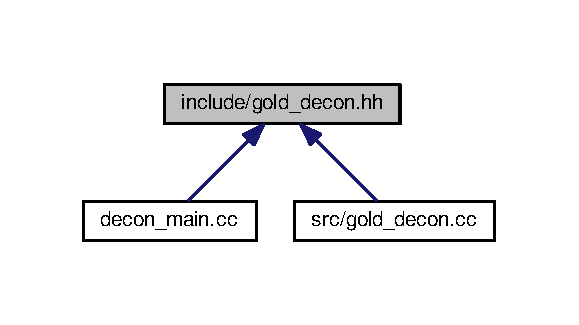
\includegraphics[width=278pt]{gold__decon_8hh__dep__incl}
\end{center}
\end{figure}
\subsection*{Classes}
\begin{DoxyCompactItemize}
\item 
class \mbox{\hyperlink{classgold__decon}{gold\+\_\+decon}}
\end{DoxyCompactItemize}
\subsection*{Variables}
\begin{DoxyCompactItemize}
\item 
int \mbox{\hyperlink{gold__decon_8hh_ab96841bb4729a804d76a68a015d1df14}{iso\+\_\+count}}
\end{DoxyCompactItemize}


\subsection{Variable Documentation}
\mbox{\Hypertarget{gold__decon_8hh_ab96841bb4729a804d76a68a015d1df14}\label{gold__decon_8hh_ab96841bb4729a804d76a68a015d1df14}} 
\index{gold\+\_\+decon.\+hh@{gold\+\_\+decon.\+hh}!iso\+\_\+count@{iso\+\_\+count}}
\index{iso\+\_\+count@{iso\+\_\+count}!gold\+\_\+decon.\+hh@{gold\+\_\+decon.\+hh}}
\subsubsection{\texorpdfstring{iso\+\_\+count}{iso\_count}}
{\footnotesize\ttfamily int iso\+\_\+count}


\hypertarget{histo_8hh}{}\section{include/histo.hh File Reference}
\label{histo_8hh}\index{include/histo.\+hh@{include/histo.\+hh}}
This graph shows which files directly or indirectly include this file\+:
\nopagebreak
\begin{figure}[H]
\begin{center}
\leavevmode
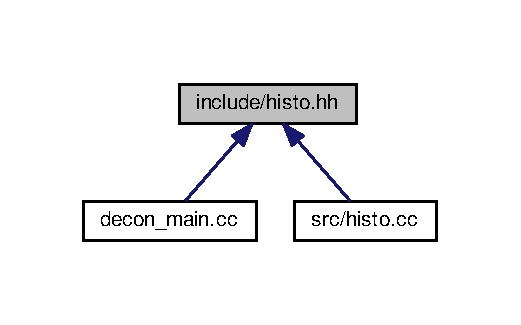
\includegraphics[width=250pt]{histo_8hh__dep__incl}
\end{center}
\end{figure}
\subsection*{Classes}
\begin{DoxyCompactItemize}
\item 
class \mbox{\hyperlink{classhisto}{histo}}
\end{DoxyCompactItemize}
\subsection*{Variables}
\begin{DoxyCompactItemize}
\item 
float \mbox{\hyperlink{histo_8hh_a43cce2495419f8219330c5474b026242}{source\+\_\+decon}} \mbox{[}4096\mbox{]}
\end{DoxyCompactItemize}


\subsection{Variable Documentation}
\mbox{\Hypertarget{histo_8hh_a43cce2495419f8219330c5474b026242}\label{histo_8hh_a43cce2495419f8219330c5474b026242}} 
\index{histo.\+hh@{histo.\+hh}!source\+\_\+decon@{source\+\_\+decon}}
\index{source\+\_\+decon@{source\+\_\+decon}!histo.\+hh@{histo.\+hh}}
\subsubsection{\texorpdfstring{source\+\_\+decon}{source\_decon}}
{\footnotesize\ttfamily float source\+\_\+decon\mbox{[}4096\mbox{]}}


\hypertarget{resp__read_8hh}{}\section{include/resp\+\_\+read.hh File Reference}
\label{resp__read_8hh}\index{include/resp\+\_\+read.\+hh@{include/resp\+\_\+read.\+hh}}
This graph shows which files directly or indirectly include this file\+:
\nopagebreak
\begin{figure}[H]
\begin{center}
\leavevmode
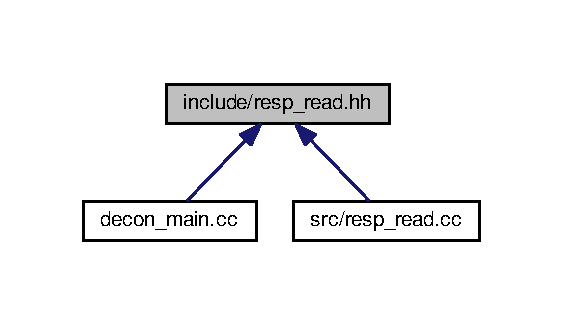
\includegraphics[width=270pt]{resp__read_8hh__dep__incl}
\end{center}
\end{figure}
\subsection*{Classes}
\begin{DoxyCompactItemize}
\item 
class \mbox{\hyperlink{classresp__read}{resp\+\_\+read}}
\end{DoxyCompactItemize}
\subsection*{Variables}
\begin{DoxyCompactItemize}
\item 
std\+::vector$<$ std\+::vector$<$ float $>$ $>$ \mbox{\hyperlink{resp__read_8hh_a1576c0eb61bce8dc9a09e20cbf5827f7}{resp\+\_\+mat\+\_\+read}}
\item 
std\+::vector$<$ float $>$ \mbox{\hyperlink{resp__read_8hh_a442adefcbd178422c9eedf7ba7860f9b}{resp\+\_\+space\+\_\+mat\+\_\+read}}
\end{DoxyCompactItemize}


\subsection{Variable Documentation}
\mbox{\Hypertarget{resp__read_8hh_a1576c0eb61bce8dc9a09e20cbf5827f7}\label{resp__read_8hh_a1576c0eb61bce8dc9a09e20cbf5827f7}} 
\index{resp\+\_\+read.\+hh@{resp\+\_\+read.\+hh}!resp\+\_\+mat\+\_\+read@{resp\+\_\+mat\+\_\+read}}
\index{resp\+\_\+mat\+\_\+read@{resp\+\_\+mat\+\_\+read}!resp\+\_\+read.\+hh@{resp\+\_\+read.\+hh}}
\subsubsection{\texorpdfstring{resp\+\_\+mat\+\_\+read}{resp\_mat\_read}}
{\footnotesize\ttfamily std\+::vector$<$std\+::vector $<$float$>$ $>$ resp\+\_\+mat\+\_\+read}

\mbox{\Hypertarget{resp__read_8hh_a442adefcbd178422c9eedf7ba7860f9b}\label{resp__read_8hh_a442adefcbd178422c9eedf7ba7860f9b}} 
\index{resp\+\_\+read.\+hh@{resp\+\_\+read.\+hh}!resp\+\_\+space\+\_\+mat\+\_\+read@{resp\+\_\+space\+\_\+mat\+\_\+read}}
\index{resp\+\_\+space\+\_\+mat\+\_\+read@{resp\+\_\+space\+\_\+mat\+\_\+read}!resp\+\_\+read.\+hh@{resp\+\_\+read.\+hh}}
\subsubsection{\texorpdfstring{resp\+\_\+space\+\_\+mat\+\_\+read}{resp\_space\_mat\_read}}
{\footnotesize\ttfamily std\+::vector$<$float$>$ resp\+\_\+space\+\_\+mat\+\_\+read}


\hypertarget{sim__source_8hh}{}\section{include/sim\+\_\+source.hh File Reference}
\label{sim__source_8hh}\index{include/sim\+\_\+source.\+hh@{include/sim\+\_\+source.\+hh}}
This graph shows which files directly or indirectly include this file\+:
\nopagebreak
\begin{figure}[H]
\begin{center}
\leavevmode
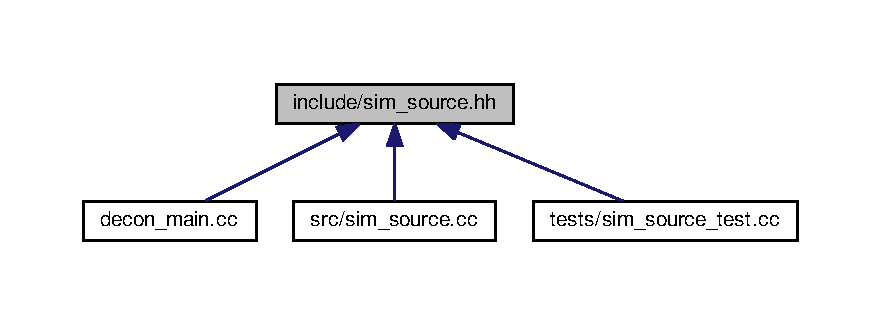
\includegraphics[width=350pt]{sim__source_8hh__dep__incl}
\end{center}
\end{figure}
\subsection*{Classes}
\begin{DoxyCompactItemize}
\item 
class \mbox{\hyperlink{classsim__source}{sim\+\_\+source}}
\end{DoxyCompactItemize}
\subsection*{Variables}
\begin{DoxyCompactItemize}
\item 
std\+::vector$<$ float $>$ \mbox{\hyperlink{sim__source_8hh_a49b7c5a2a0c45a7030e935e2b212d26f}{data\+\_\+sim}}
\item 
std\+::vector$<$ std\+::vector$<$ float $>$ $>$ \mbox{\hyperlink{sim__source_8hh_a98a2ef7afad727679ee5c11bd6cc4df0}{space\+\_\+sim}}
\end{DoxyCompactItemize}


\subsection{Variable Documentation}
\mbox{\Hypertarget{sim__source_8hh_a49b7c5a2a0c45a7030e935e2b212d26f}\label{sim__source_8hh_a49b7c5a2a0c45a7030e935e2b212d26f}} 
\index{sim\+\_\+source.\+hh@{sim\+\_\+source.\+hh}!data\+\_\+sim@{data\+\_\+sim}}
\index{data\+\_\+sim@{data\+\_\+sim}!sim\+\_\+source.\+hh@{sim\+\_\+source.\+hh}}
\subsubsection{\texorpdfstring{data\+\_\+sim}{data\_sim}}
{\footnotesize\ttfamily std\+::vector$<$float$>$ data\+\_\+sim}

\mbox{\Hypertarget{sim__source_8hh_a98a2ef7afad727679ee5c11bd6cc4df0}\label{sim__source_8hh_a98a2ef7afad727679ee5c11bd6cc4df0}} 
\index{sim\+\_\+source.\+hh@{sim\+\_\+source.\+hh}!space\+\_\+sim@{space\+\_\+sim}}
\index{space\+\_\+sim@{space\+\_\+sim}!sim\+\_\+source.\+hh@{sim\+\_\+source.\+hh}}
\subsubsection{\texorpdfstring{space\+\_\+sim}{space\_sim}}
{\footnotesize\ttfamily std\+::vector$<$ std\+::vector$<$float$>$ $>$ space\+\_\+sim}


\hypertarget{spatial__decon_8hh}{}\section{include/spatial\+\_\+decon.hh File Reference}
\label{spatial__decon_8hh}\index{include/spatial\+\_\+decon.\+hh@{include/spatial\+\_\+decon.\+hh}}
This graph shows which files directly or indirectly include this file\+:
\nopagebreak
\begin{figure}[H]
\begin{center}
\leavevmode
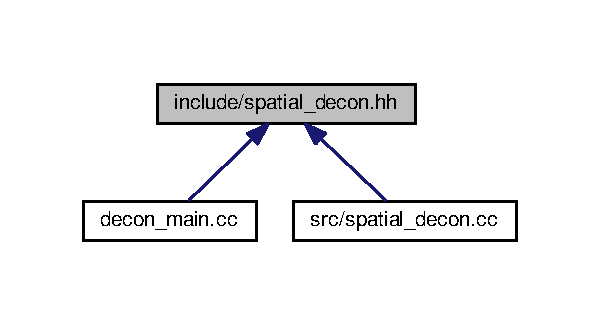
\includegraphics[width=288pt]{spatial__decon_8hh__dep__incl}
\end{center}
\end{figure}
\subsection*{Classes}
\begin{DoxyCompactItemize}
\item 
class \mbox{\hyperlink{classspatial__decon}{spatial\+\_\+decon}}
\end{DoxyCompactItemize}
\subsection*{Variables}
\begin{DoxyCompactItemize}
\item 
std\+::vector$<$ std\+::vector$<$ int $>$ $>$ \mbox{\hyperlink{spatial__decon_8hh_a3256ec6aeca97c99b8e9901bfda6e9ab}{end\+\_\+ind}}
\end{DoxyCompactItemize}


\subsection{Variable Documentation}
\mbox{\Hypertarget{spatial__decon_8hh_a3256ec6aeca97c99b8e9901bfda6e9ab}\label{spatial__decon_8hh_a3256ec6aeca97c99b8e9901bfda6e9ab}} 
\index{spatial\+\_\+decon.\+hh@{spatial\+\_\+decon.\+hh}!end\+\_\+ind@{end\+\_\+ind}}
\index{end\+\_\+ind@{end\+\_\+ind}!spatial\+\_\+decon.\+hh@{spatial\+\_\+decon.\+hh}}
\subsubsection{\texorpdfstring{end\+\_\+ind}{end\_ind}}
{\footnotesize\ttfamily std\+::vector$<$ std\+::vector$<$int$>$ $>$ end\+\_\+ind}


\hypertarget{readme_8md}{}\section{readme.\+md File Reference}
\label{readme_8md}\index{readme.\+md@{readme.\+md}}

\hypertarget{source_sim3_8m}{}\section{source\+\_\+sims/source\+Sim3.m File Reference}
\label{source_sim3_8m}\index{source\+\_\+sims/source\+Sim3.\+m@{source\+\_\+sims/source\+Sim3.\+m}}
\subsection*{Functions}
\begin{DoxyCompactItemize}
\item 
function \mbox{\hyperlink{source_sim3_8m_aa9c015bb163079debe4c44838417f65b}{source\+Sim}} () f\+I\+Dsum
\item 
end \mbox{\hyperlink{source_sim3_8m_a3d41fb1c1d215d6a65f9ca175ed1e820}{plot}} (1\+:4096, \mbox{\hyperlink{source_sim3_8m_ab9000230b7c99413cc499423d7834e01}{spect\+Sim}}) fprintf(f\+I\+Dsum
\item 
\mbox{\hyperlink{source_sim3_8m_a1ed8d630c4de63ab7d3cec40e09718cb}{fclose}} (\textquotesingle{}all\textquotesingle{})
\end{DoxyCompactItemize}
\subsection*{Variables}
\begin{DoxyCompactItemize}
\item 
\mbox{\hyperlink{source_sim3_8m_a5ee06caf276e5e1efe034c6af062bf7c}{f\+I\+D1}} = fopen(\textquotesingle{}2\+\_\+21\+\_\+am241.\+txt\textquotesingle{}, \textquotesingle{}r\textquotesingle{})
\item 
\mbox{\hyperlink{source_sim3_8m_a46174c6aae0948a5fd43ac934f9f1d74}{f\+I\+D2}} = fopen(\textquotesingle{}2\+\_\+21\+\_\+co60.\+txt\textquotesingle{}, \textquotesingle{}r\textquotesingle{})
\item 
\mbox{\hyperlink{source_sim3_8m_a4cf3119830cb79f2d0bce3c5047c046c}{f\+I\+D3}} = fopen(\textquotesingle{}2\+\_\+21\+\_\+nat\+U.\+txt\textquotesingle{}, \textquotesingle{}r\textquotesingle{})
\item 
\mbox{\hyperlink{source_sim3_8m_a2c76e01a360f7d86a3745d6e94a3df1b}{f\+I\+D4}} = fopen(\textquotesingle{}2\+\_\+21\+\_\+ra226.\+txt\textquotesingle{}, \textquotesingle{}r\textquotesingle{})
\item 
\mbox{\hyperlink{source_sim3_8m_abf0ba3c9f2e33eca973a0ab956722520}{f\+I\+D5}} = fopen(\textquotesingle{}2\+\_\+21\+\_\+cs137.\+txt\textquotesingle{}, \textquotesingle{}r\textquotesingle{})
\item 
\mbox{\hyperlink{source_sim3_8m_a827bd6f5b1b95f5edc6d52a706af7b4c}{f\+I\+D6}} = fopen(\textquotesingle{}2\+\_\+21\+\_\+hour\+\_\+\+B\+G.\+txt\textquotesingle{}, \textquotesingle{}r\textquotesingle{})
\item 
\mbox{\hyperlink{source_sim3_8m_a195632020137a1d2a23f270b0162fb96}{f\+I\+D7}} = fopen(\textquotesingle{}3\+\_\+1\+\_\+bkg.\+txt\textquotesingle{}, \textquotesingle{}r\textquotesingle{})
\item 
\mbox{\hyperlink{source_sim3_8m_a79de9c5adaa0819746ab52408c2a06ca}{f\+I\+D8}} = fopen(\textquotesingle{}3\+\_\+28\+\_\+am241\+\_\+2hr.\+txt\textquotesingle{}, \textquotesingle{}r\textquotesingle{})
\item 
\mbox{\hyperlink{source_sim3_8m_a71f0988cc51311e5c6988610aa57cb41}{f\+I\+D9}} = fopen(\textquotesingle{}3\+\_\+28\+\_\+ntrl\+U\+\_\+2hr.\+txt\textquotesingle{}, \textquotesingle{}r\textquotesingle{})
\item 
\mbox{\hyperlink{source_sim3_8m_a598f8f64c3d39d1971c5b8cafb901688}{f\+I\+D10}} = fopen(\textquotesingle{}3\+\_\+28\+\_\+u235\+\_\+2hr.\+txt\textquotesingle{}, \textquotesingle{}r\textquotesingle{})
\item 
\mbox{\hyperlink{source_sim3_8m_adbfe3622d2915b74209739ec11aefefd}{f\+I\+D11}} = fopen(\textquotesingle{}3\+\_\+29\+\_\+co6\+\_\+2hr.\+txt\textquotesingle{}, \textquotesingle{}r\textquotesingle{})
\item 
\mbox{\hyperlink{source_sim3_8m_a29eb24d2e2d3579e0f5f3c7f4a75af84}{f\+I\+D12}} = fopen(\textquotesingle{}3\+\_\+29\+\_\+ra226\+\_\+2hr.\+txt\textquotesingle{}, \textquotesingle{}r\textquotesingle{})
\item 
\mbox{\hyperlink{source_sim3_8m_adf77711285ca752c9cac974bf8a028f0}{f\+I\+D13}} = fopen(\textquotesingle{}3\+\_\+28\+\_\+bkg\+\_\+12hr.\+txt\textquotesingle{}, \textquotesingle{}r\textquotesingle{})
\item 
\mbox{\hyperlink{source_sim3_8m_a713778b7970b96145d59957fe8cb7de6}{spect1}} = fscanf(\mbox{\hyperlink{source_sim3_8m_a5ee06caf276e5e1efe034c6af062bf7c}{f\+I\+D1}}, \textquotesingle{}\%f\textquotesingle{})
\item 
\mbox{\hyperlink{source_sim3_8m_a0861067e480539b6debeb52839e2a6e2}{spect2}} = fscanf(\mbox{\hyperlink{source_sim3_8m_a46174c6aae0948a5fd43ac934f9f1d74}{f\+I\+D2}}, \textquotesingle{}\%f\textquotesingle{})
\item 
\mbox{\hyperlink{source_sim3_8m_a8e22fcde0d07a27c28d94b833d4f6527}{spect3}} = fscanf(\mbox{\hyperlink{source_sim3_8m_a4cf3119830cb79f2d0bce3c5047c046c}{f\+I\+D3}}, \textquotesingle{}\%f\textquotesingle{})
\item 
\mbox{\hyperlink{source_sim3_8m_aea58e9a851c66a8cce7a19f8bb3f7592}{spect4}} = fscanf(\mbox{\hyperlink{source_sim3_8m_a2c76e01a360f7d86a3745d6e94a3df1b}{f\+I\+D4}}, \textquotesingle{}\%f\textquotesingle{})
\item 
\mbox{\hyperlink{source_sim3_8m_ab2cca27f08b384101540743b0b796c09}{spect5}} = fscanf(\mbox{\hyperlink{source_sim3_8m_abf0ba3c9f2e33eca973a0ab956722520}{f\+I\+D5}}, \textquotesingle{}\%f\textquotesingle{})
\item 
\mbox{\hyperlink{source_sim3_8m_a1ab0a5da677feb9c361f3cd3658a5172}{spect6}} = fscanf(\mbox{\hyperlink{source_sim3_8m_a827bd6f5b1b95f5edc6d52a706af7b4c}{f\+I\+D6}}, \textquotesingle{}\%f\textquotesingle{})
\item 
\mbox{\hyperlink{source_sim3_8m_abbb46808b3b8ebde7500f31f2d76dda9}{spect7}} = fscanf(\mbox{\hyperlink{source_sim3_8m_a195632020137a1d2a23f270b0162fb96}{f\+I\+D7}}, \textquotesingle{}\%f\textquotesingle{})
\item 
\mbox{\hyperlink{source_sim3_8m_aa73cabe3a58d555c1b2b47881e0fe8d9}{spect8}} = fscanf(\mbox{\hyperlink{source_sim3_8m_a79de9c5adaa0819746ab52408c2a06ca}{f\+I\+D8}}, \textquotesingle{}\%f\textquotesingle{})
\item 
\mbox{\hyperlink{source_sim3_8m_a90a81415859956adea89fb14d03a9172}{spect9}} = fscanf(\mbox{\hyperlink{source_sim3_8m_a71f0988cc51311e5c6988610aa57cb41}{f\+I\+D9}}, \textquotesingle{}\%f\textquotesingle{})
\item 
\mbox{\hyperlink{source_sim3_8m_a021ebf166ed2b81bd3afb2938a028327}{spect10}} = fscanf(\mbox{\hyperlink{source_sim3_8m_a598f8f64c3d39d1971c5b8cafb901688}{f\+I\+D10}}, \textquotesingle{}\%f\textquotesingle{})
\item 
\mbox{\hyperlink{source_sim3_8m_a7045441c130209ced5e6fe716b40fef0}{spect11}} = fscanf(\mbox{\hyperlink{source_sim3_8m_adbfe3622d2915b74209739ec11aefefd}{f\+I\+D11}}, \textquotesingle{}\%f\textquotesingle{})
\item 
\mbox{\hyperlink{source_sim3_8m_acedaf16d287b949145738e2e4c9295d8}{spect12}} = fscanf(\mbox{\hyperlink{source_sim3_8m_a29eb24d2e2d3579e0f5f3c7f4a75af84}{f\+I\+D12}}, \textquotesingle{}\%f\textquotesingle{})
\item 
\mbox{\hyperlink{source_sim3_8m_a8792d47cae96de1d3646035fa5c5e47e}{spect13}} = fscanf(\mbox{\hyperlink{source_sim3_8m_adf77711285ca752c9cac974bf8a028f0}{f\+I\+D13}}, \textquotesingle{}\%f\textquotesingle{})
\item 
\mbox{\hyperlink{source_sim3_8m_ab9000230b7c99413cc499423d7834e01}{spect\+Sim}} = \mbox{[}$\,$\mbox{]}
\item 
\mbox{\hyperlink{source__read_8cc_a816e149c6568a71e8b4e60e91677df90}{for}} \mbox{\hyperlink{source_sim3_8m_a6f6ccfcf58b31cb6412107d9d5281426}{i}}
\item 
Spect Set \mbox{\hyperlink{source_sim3_8m_a0200868083bda21e2c57e7f40c1c1d63}{sum\+Spect}} = sum\+Spect + round(0 $\ast$ \mbox{\hyperlink{source_sim3_8m_a713778b7970b96145d59957fe8cb7de6}{spect1}}(\mbox{\hyperlink{source_sim3_8m_a6f6ccfcf58b31cb6412107d9d5281426}{i}}) / (2 $\ast$ 60))
\item 
end \mbox{\hyperlink{source_sim3_8m_a6f6ccfcf58b31cb6412107d9d5281426}{i}} \mbox{\hyperlink{source_sim3_8m_afde56a346740bd8c5e1e00304507601d}{n}}
\end{DoxyCompactItemize}


\subsection{Function Documentation}
\mbox{\Hypertarget{source_sim3_8m_a1ed8d630c4de63ab7d3cec40e09718cb}\label{source_sim3_8m_a1ed8d630c4de63ab7d3cec40e09718cb}} 
\index{source\+Sim3.\+m@{source\+Sim3.\+m}!fclose@{fclose}}
\index{fclose@{fclose}!source\+Sim3.\+m@{source\+Sim3.\+m}}
\subsubsection{\texorpdfstring{fclose()}{fclose()}}
{\footnotesize\ttfamily fclose (\begin{DoxyParamCaption}\item[{\textquotesingle{}all\textquotesingle{}}]{ }\end{DoxyParamCaption})}

\mbox{\Hypertarget{source_sim3_8m_a3d41fb1c1d215d6a65f9ca175ed1e820}\label{source_sim3_8m_a3d41fb1c1d215d6a65f9ca175ed1e820}} 
\index{source\+Sim3.\+m@{source\+Sim3.\+m}!plot@{plot}}
\index{plot@{plot}!source\+Sim3.\+m@{source\+Sim3.\+m}}
\subsubsection{\texorpdfstring{plot()}{plot()}}
{\footnotesize\ttfamily end plot (\begin{DoxyParamCaption}\item[{1\+:4096}]{,  }\item[{\mbox{\hyperlink{source_sim3_8m_ab9000230b7c99413cc499423d7834e01}{spect\+Sim}}}]{ }\end{DoxyParamCaption})}

\mbox{\Hypertarget{source_sim3_8m_aa9c015bb163079debe4c44838417f65b}\label{source_sim3_8m_aa9c015bb163079debe4c44838417f65b}} 
\index{source\+Sim3.\+m@{source\+Sim3.\+m}!source\+Sim@{source\+Sim}}
\index{source\+Sim@{source\+Sim}!source\+Sim3.\+m@{source\+Sim3.\+m}}
\subsubsection{\texorpdfstring{source\+Sim()}{sourceSim()}}
{\footnotesize\ttfamily function source\+Sim (\begin{DoxyParamCaption}{ }\end{DoxyParamCaption})}



\subsection{Variable Documentation}
\mbox{\Hypertarget{source_sim3_8m_a5ee06caf276e5e1efe034c6af062bf7c}\label{source_sim3_8m_a5ee06caf276e5e1efe034c6af062bf7c}} 
\index{source\+Sim3.\+m@{source\+Sim3.\+m}!f\+I\+D1@{f\+I\+D1}}
\index{f\+I\+D1@{f\+I\+D1}!source\+Sim3.\+m@{source\+Sim3.\+m}}
\subsubsection{\texorpdfstring{f\+I\+D1}{fID1}}
{\footnotesize\ttfamily f\+I\+D1 = fopen(\textquotesingle{}2\+\_\+21\+\_\+am241.\+txt\textquotesingle{}, \textquotesingle{}r\textquotesingle{})}

\mbox{\Hypertarget{source_sim3_8m_a598f8f64c3d39d1971c5b8cafb901688}\label{source_sim3_8m_a598f8f64c3d39d1971c5b8cafb901688}} 
\index{source\+Sim3.\+m@{source\+Sim3.\+m}!f\+I\+D10@{f\+I\+D10}}
\index{f\+I\+D10@{f\+I\+D10}!source\+Sim3.\+m@{source\+Sim3.\+m}}
\subsubsection{\texorpdfstring{f\+I\+D10}{fID10}}
{\footnotesize\ttfamily f\+I\+D10 = fopen(\textquotesingle{}3\+\_\+28\+\_\+u235\+\_\+2hr.\+txt\textquotesingle{}, \textquotesingle{}r\textquotesingle{})}

\mbox{\Hypertarget{source_sim3_8m_adbfe3622d2915b74209739ec11aefefd}\label{source_sim3_8m_adbfe3622d2915b74209739ec11aefefd}} 
\index{source\+Sim3.\+m@{source\+Sim3.\+m}!f\+I\+D11@{f\+I\+D11}}
\index{f\+I\+D11@{f\+I\+D11}!source\+Sim3.\+m@{source\+Sim3.\+m}}
\subsubsection{\texorpdfstring{f\+I\+D11}{fID11}}
{\footnotesize\ttfamily f\+I\+D11 = fopen(\textquotesingle{}3\+\_\+29\+\_\+co6\+\_\+2hr.\+txt\textquotesingle{}, \textquotesingle{}r\textquotesingle{})}

\mbox{\Hypertarget{source_sim3_8m_a29eb24d2e2d3579e0f5f3c7f4a75af84}\label{source_sim3_8m_a29eb24d2e2d3579e0f5f3c7f4a75af84}} 
\index{source\+Sim3.\+m@{source\+Sim3.\+m}!f\+I\+D12@{f\+I\+D12}}
\index{f\+I\+D12@{f\+I\+D12}!source\+Sim3.\+m@{source\+Sim3.\+m}}
\subsubsection{\texorpdfstring{f\+I\+D12}{fID12}}
{\footnotesize\ttfamily f\+I\+D12 = fopen(\textquotesingle{}3\+\_\+29\+\_\+ra226\+\_\+2hr.\+txt\textquotesingle{}, \textquotesingle{}r\textquotesingle{})}

\mbox{\Hypertarget{source_sim3_8m_adf77711285ca752c9cac974bf8a028f0}\label{source_sim3_8m_adf77711285ca752c9cac974bf8a028f0}} 
\index{source\+Sim3.\+m@{source\+Sim3.\+m}!f\+I\+D13@{f\+I\+D13}}
\index{f\+I\+D13@{f\+I\+D13}!source\+Sim3.\+m@{source\+Sim3.\+m}}
\subsubsection{\texorpdfstring{f\+I\+D13}{fID13}}
{\footnotesize\ttfamily f\+I\+D13 = fopen(\textquotesingle{}3\+\_\+28\+\_\+bkg\+\_\+12hr.\+txt\textquotesingle{}, \textquotesingle{}r\textquotesingle{})}

\mbox{\Hypertarget{source_sim3_8m_a46174c6aae0948a5fd43ac934f9f1d74}\label{source_sim3_8m_a46174c6aae0948a5fd43ac934f9f1d74}} 
\index{source\+Sim3.\+m@{source\+Sim3.\+m}!f\+I\+D2@{f\+I\+D2}}
\index{f\+I\+D2@{f\+I\+D2}!source\+Sim3.\+m@{source\+Sim3.\+m}}
\subsubsection{\texorpdfstring{f\+I\+D2}{fID2}}
{\footnotesize\ttfamily f\+I\+D2 = fopen(\textquotesingle{}2\+\_\+21\+\_\+co60.\+txt\textquotesingle{}, \textquotesingle{}r\textquotesingle{})}

\mbox{\Hypertarget{source_sim3_8m_a4cf3119830cb79f2d0bce3c5047c046c}\label{source_sim3_8m_a4cf3119830cb79f2d0bce3c5047c046c}} 
\index{source\+Sim3.\+m@{source\+Sim3.\+m}!f\+I\+D3@{f\+I\+D3}}
\index{f\+I\+D3@{f\+I\+D3}!source\+Sim3.\+m@{source\+Sim3.\+m}}
\subsubsection{\texorpdfstring{f\+I\+D3}{fID3}}
{\footnotesize\ttfamily f\+I\+D3 = fopen(\textquotesingle{}2\+\_\+21\+\_\+nat\+U.\+txt\textquotesingle{}, \textquotesingle{}r\textquotesingle{})}

\mbox{\Hypertarget{source_sim3_8m_a2c76e01a360f7d86a3745d6e94a3df1b}\label{source_sim3_8m_a2c76e01a360f7d86a3745d6e94a3df1b}} 
\index{source\+Sim3.\+m@{source\+Sim3.\+m}!f\+I\+D4@{f\+I\+D4}}
\index{f\+I\+D4@{f\+I\+D4}!source\+Sim3.\+m@{source\+Sim3.\+m}}
\subsubsection{\texorpdfstring{f\+I\+D4}{fID4}}
{\footnotesize\ttfamily f\+I\+D4 = fopen(\textquotesingle{}2\+\_\+21\+\_\+ra226.\+txt\textquotesingle{}, \textquotesingle{}r\textquotesingle{})}

\mbox{\Hypertarget{source_sim3_8m_abf0ba3c9f2e33eca973a0ab956722520}\label{source_sim3_8m_abf0ba3c9f2e33eca973a0ab956722520}} 
\index{source\+Sim3.\+m@{source\+Sim3.\+m}!f\+I\+D5@{f\+I\+D5}}
\index{f\+I\+D5@{f\+I\+D5}!source\+Sim3.\+m@{source\+Sim3.\+m}}
\subsubsection{\texorpdfstring{f\+I\+D5}{fID5}}
{\footnotesize\ttfamily f\+I\+D5 = fopen(\textquotesingle{}2\+\_\+21\+\_\+cs137.\+txt\textquotesingle{}, \textquotesingle{}r\textquotesingle{})}

\mbox{\Hypertarget{source_sim3_8m_a827bd6f5b1b95f5edc6d52a706af7b4c}\label{source_sim3_8m_a827bd6f5b1b95f5edc6d52a706af7b4c}} 
\index{source\+Sim3.\+m@{source\+Sim3.\+m}!f\+I\+D6@{f\+I\+D6}}
\index{f\+I\+D6@{f\+I\+D6}!source\+Sim3.\+m@{source\+Sim3.\+m}}
\subsubsection{\texorpdfstring{f\+I\+D6}{fID6}}
{\footnotesize\ttfamily f\+I\+D6 = fopen(\textquotesingle{}2\+\_\+21\+\_\+hour\+\_\+\+B\+G.\+txt\textquotesingle{}, \textquotesingle{}r\textquotesingle{})}

\mbox{\Hypertarget{source_sim3_8m_a195632020137a1d2a23f270b0162fb96}\label{source_sim3_8m_a195632020137a1d2a23f270b0162fb96}} 
\index{source\+Sim3.\+m@{source\+Sim3.\+m}!f\+I\+D7@{f\+I\+D7}}
\index{f\+I\+D7@{f\+I\+D7}!source\+Sim3.\+m@{source\+Sim3.\+m}}
\subsubsection{\texorpdfstring{f\+I\+D7}{fID7}}
{\footnotesize\ttfamily f\+I\+D7 = fopen(\textquotesingle{}3\+\_\+1\+\_\+bkg.\+txt\textquotesingle{}, \textquotesingle{}r\textquotesingle{})}

\mbox{\Hypertarget{source_sim3_8m_a79de9c5adaa0819746ab52408c2a06ca}\label{source_sim3_8m_a79de9c5adaa0819746ab52408c2a06ca}} 
\index{source\+Sim3.\+m@{source\+Sim3.\+m}!f\+I\+D8@{f\+I\+D8}}
\index{f\+I\+D8@{f\+I\+D8}!source\+Sim3.\+m@{source\+Sim3.\+m}}
\subsubsection{\texorpdfstring{f\+I\+D8}{fID8}}
{\footnotesize\ttfamily f\+I\+D8 = fopen(\textquotesingle{}3\+\_\+28\+\_\+am241\+\_\+2hr.\+txt\textquotesingle{}, \textquotesingle{}r\textquotesingle{})}

\mbox{\Hypertarget{source_sim3_8m_a71f0988cc51311e5c6988610aa57cb41}\label{source_sim3_8m_a71f0988cc51311e5c6988610aa57cb41}} 
\index{source\+Sim3.\+m@{source\+Sim3.\+m}!f\+I\+D9@{f\+I\+D9}}
\index{f\+I\+D9@{f\+I\+D9}!source\+Sim3.\+m@{source\+Sim3.\+m}}
\subsubsection{\texorpdfstring{f\+I\+D9}{fID9}}
{\footnotesize\ttfamily f\+I\+D9 = fopen(\textquotesingle{}3\+\_\+28\+\_\+ntrl\+U\+\_\+2hr.\+txt\textquotesingle{}, \textquotesingle{}r\textquotesingle{})}

\mbox{\Hypertarget{source_sim3_8m_a6f6ccfcf58b31cb6412107d9d5281426}\label{source_sim3_8m_a6f6ccfcf58b31cb6412107d9d5281426}} 
\index{source\+Sim3.\+m@{source\+Sim3.\+m}!i@{i}}
\index{i@{i}!source\+Sim3.\+m@{source\+Sim3.\+m}}
\subsubsection{\texorpdfstring{i}{i}}
{\footnotesize\ttfamily \mbox{\hyperlink{source__read_8cc_a816e149c6568a71e8b4e60e91677df90}{for}} i}

{\bfseries Initial value\+:}
\begin{DoxyCode}
=1:4096
        
        \mbox{\hyperlink{source_sim3_8m_a0200868083bda21e2c57e7f40c1c1d63}{sumSpect}} = 0
\end{DoxyCode}
\mbox{\Hypertarget{source_sim3_8m_afde56a346740bd8c5e1e00304507601d}\label{source_sim3_8m_afde56a346740bd8c5e1e00304507601d}} 
\index{source\+Sim3.\+m@{source\+Sim3.\+m}!n@{n}}
\index{n@{n}!source\+Sim3.\+m@{source\+Sim3.\+m}}
\subsubsection{\texorpdfstring{n}{n}}
{\footnotesize\ttfamily end \mbox{\hyperlink{source_sim3_8m_a6f6ccfcf58b31cb6412107d9d5281426}{i}} n}

\mbox{\Hypertarget{source_sim3_8m_a713778b7970b96145d59957fe8cb7de6}\label{source_sim3_8m_a713778b7970b96145d59957fe8cb7de6}} 
\index{source\+Sim3.\+m@{source\+Sim3.\+m}!spect1@{spect1}}
\index{spect1@{spect1}!source\+Sim3.\+m@{source\+Sim3.\+m}}
\subsubsection{\texorpdfstring{spect1}{spect1}}
{\footnotesize\ttfamily spect1 = fscanf(\mbox{\hyperlink{source_sim3_8m_a5ee06caf276e5e1efe034c6af062bf7c}{f\+I\+D1}}, \textquotesingle{}\%f\textquotesingle{})}

\mbox{\Hypertarget{source_sim3_8m_a021ebf166ed2b81bd3afb2938a028327}\label{source_sim3_8m_a021ebf166ed2b81bd3afb2938a028327}} 
\index{source\+Sim3.\+m@{source\+Sim3.\+m}!spect10@{spect10}}
\index{spect10@{spect10}!source\+Sim3.\+m@{source\+Sim3.\+m}}
\subsubsection{\texorpdfstring{spect10}{spect10}}
{\footnotesize\ttfamily spect10 = fscanf(\mbox{\hyperlink{source_sim3_8m_a598f8f64c3d39d1971c5b8cafb901688}{f\+I\+D10}}, \textquotesingle{}\%f\textquotesingle{})}

\mbox{\Hypertarget{source_sim3_8m_a7045441c130209ced5e6fe716b40fef0}\label{source_sim3_8m_a7045441c130209ced5e6fe716b40fef0}} 
\index{source\+Sim3.\+m@{source\+Sim3.\+m}!spect11@{spect11}}
\index{spect11@{spect11}!source\+Sim3.\+m@{source\+Sim3.\+m}}
\subsubsection{\texorpdfstring{spect11}{spect11}}
{\footnotesize\ttfamily spect11 = fscanf(\mbox{\hyperlink{source_sim3_8m_adbfe3622d2915b74209739ec11aefefd}{f\+I\+D11}}, \textquotesingle{}\%f\textquotesingle{})}

\mbox{\Hypertarget{source_sim3_8m_acedaf16d287b949145738e2e4c9295d8}\label{source_sim3_8m_acedaf16d287b949145738e2e4c9295d8}} 
\index{source\+Sim3.\+m@{source\+Sim3.\+m}!spect12@{spect12}}
\index{spect12@{spect12}!source\+Sim3.\+m@{source\+Sim3.\+m}}
\subsubsection{\texorpdfstring{spect12}{spect12}}
{\footnotesize\ttfamily spect12 = fscanf(\mbox{\hyperlink{source_sim3_8m_a29eb24d2e2d3579e0f5f3c7f4a75af84}{f\+I\+D12}}, \textquotesingle{}\%f\textquotesingle{})}

\mbox{\Hypertarget{source_sim3_8m_a8792d47cae96de1d3646035fa5c5e47e}\label{source_sim3_8m_a8792d47cae96de1d3646035fa5c5e47e}} 
\index{source\+Sim3.\+m@{source\+Sim3.\+m}!spect13@{spect13}}
\index{spect13@{spect13}!source\+Sim3.\+m@{source\+Sim3.\+m}}
\subsubsection{\texorpdfstring{spect13}{spect13}}
{\footnotesize\ttfamily spect13 = fscanf(\mbox{\hyperlink{source_sim3_8m_adf77711285ca752c9cac974bf8a028f0}{f\+I\+D13}}, \textquotesingle{}\%f\textquotesingle{})}

\mbox{\Hypertarget{source_sim3_8m_a0861067e480539b6debeb52839e2a6e2}\label{source_sim3_8m_a0861067e480539b6debeb52839e2a6e2}} 
\index{source\+Sim3.\+m@{source\+Sim3.\+m}!spect2@{spect2}}
\index{spect2@{spect2}!source\+Sim3.\+m@{source\+Sim3.\+m}}
\subsubsection{\texorpdfstring{spect2}{spect2}}
{\footnotesize\ttfamily spect2 = fscanf(\mbox{\hyperlink{source_sim3_8m_a46174c6aae0948a5fd43ac934f9f1d74}{f\+I\+D2}}, \textquotesingle{}\%f\textquotesingle{})}

\mbox{\Hypertarget{source_sim3_8m_a8e22fcde0d07a27c28d94b833d4f6527}\label{source_sim3_8m_a8e22fcde0d07a27c28d94b833d4f6527}} 
\index{source\+Sim3.\+m@{source\+Sim3.\+m}!spect3@{spect3}}
\index{spect3@{spect3}!source\+Sim3.\+m@{source\+Sim3.\+m}}
\subsubsection{\texorpdfstring{spect3}{spect3}}
{\footnotesize\ttfamily spect3 = fscanf(\mbox{\hyperlink{source_sim3_8m_a4cf3119830cb79f2d0bce3c5047c046c}{f\+I\+D3}}, \textquotesingle{}\%f\textquotesingle{})}

\mbox{\Hypertarget{source_sim3_8m_aea58e9a851c66a8cce7a19f8bb3f7592}\label{source_sim3_8m_aea58e9a851c66a8cce7a19f8bb3f7592}} 
\index{source\+Sim3.\+m@{source\+Sim3.\+m}!spect4@{spect4}}
\index{spect4@{spect4}!source\+Sim3.\+m@{source\+Sim3.\+m}}
\subsubsection{\texorpdfstring{spect4}{spect4}}
{\footnotesize\ttfamily spect4 = fscanf(\mbox{\hyperlink{source_sim3_8m_a2c76e01a360f7d86a3745d6e94a3df1b}{f\+I\+D4}}, \textquotesingle{}\%f\textquotesingle{})}

\mbox{\Hypertarget{source_sim3_8m_ab2cca27f08b384101540743b0b796c09}\label{source_sim3_8m_ab2cca27f08b384101540743b0b796c09}} 
\index{source\+Sim3.\+m@{source\+Sim3.\+m}!spect5@{spect5}}
\index{spect5@{spect5}!source\+Sim3.\+m@{source\+Sim3.\+m}}
\subsubsection{\texorpdfstring{spect5}{spect5}}
{\footnotesize\ttfamily spect5 = fscanf(\mbox{\hyperlink{source_sim3_8m_abf0ba3c9f2e33eca973a0ab956722520}{f\+I\+D5}}, \textquotesingle{}\%f\textquotesingle{})}

\mbox{\Hypertarget{source_sim3_8m_a1ab0a5da677feb9c361f3cd3658a5172}\label{source_sim3_8m_a1ab0a5da677feb9c361f3cd3658a5172}} 
\index{source\+Sim3.\+m@{source\+Sim3.\+m}!spect6@{spect6}}
\index{spect6@{spect6}!source\+Sim3.\+m@{source\+Sim3.\+m}}
\subsubsection{\texorpdfstring{spect6}{spect6}}
{\footnotesize\ttfamily spect6 = fscanf(\mbox{\hyperlink{source_sim3_8m_a827bd6f5b1b95f5edc6d52a706af7b4c}{f\+I\+D6}}, \textquotesingle{}\%f\textquotesingle{})}

\mbox{\Hypertarget{source_sim3_8m_abbb46808b3b8ebde7500f31f2d76dda9}\label{source_sim3_8m_abbb46808b3b8ebde7500f31f2d76dda9}} 
\index{source\+Sim3.\+m@{source\+Sim3.\+m}!spect7@{spect7}}
\index{spect7@{spect7}!source\+Sim3.\+m@{source\+Sim3.\+m}}
\subsubsection{\texorpdfstring{spect7}{spect7}}
{\footnotesize\ttfamily spect7 = fscanf(\mbox{\hyperlink{source_sim3_8m_a195632020137a1d2a23f270b0162fb96}{f\+I\+D7}}, \textquotesingle{}\%f\textquotesingle{})}

\mbox{\Hypertarget{source_sim3_8m_aa73cabe3a58d555c1b2b47881e0fe8d9}\label{source_sim3_8m_aa73cabe3a58d555c1b2b47881e0fe8d9}} 
\index{source\+Sim3.\+m@{source\+Sim3.\+m}!spect8@{spect8}}
\index{spect8@{spect8}!source\+Sim3.\+m@{source\+Sim3.\+m}}
\subsubsection{\texorpdfstring{spect8}{spect8}}
{\footnotesize\ttfamily spect8 = fscanf(\mbox{\hyperlink{source_sim3_8m_a79de9c5adaa0819746ab52408c2a06ca}{f\+I\+D8}}, \textquotesingle{}\%f\textquotesingle{})}

\mbox{\Hypertarget{source_sim3_8m_a90a81415859956adea89fb14d03a9172}\label{source_sim3_8m_a90a81415859956adea89fb14d03a9172}} 
\index{source\+Sim3.\+m@{source\+Sim3.\+m}!spect9@{spect9}}
\index{spect9@{spect9}!source\+Sim3.\+m@{source\+Sim3.\+m}}
\subsubsection{\texorpdfstring{spect9}{spect9}}
{\footnotesize\ttfamily spect9 = fscanf(\mbox{\hyperlink{source_sim3_8m_a71f0988cc51311e5c6988610aa57cb41}{f\+I\+D9}}, \textquotesingle{}\%f\textquotesingle{})}

\mbox{\Hypertarget{source_sim3_8m_ab9000230b7c99413cc499423d7834e01}\label{source_sim3_8m_ab9000230b7c99413cc499423d7834e01}} 
\index{source\+Sim3.\+m@{source\+Sim3.\+m}!spect\+Sim@{spect\+Sim}}
\index{spect\+Sim@{spect\+Sim}!source\+Sim3.\+m@{source\+Sim3.\+m}}
\subsubsection{\texorpdfstring{spect\+Sim}{spectSim}}
{\footnotesize\ttfamily end \mbox{\hyperlink{source_sim3_8m_a6f6ccfcf58b31cb6412107d9d5281426}{i}} spect\+Sim = \mbox{[}$\,$\mbox{]}}

\mbox{\Hypertarget{source_sim3_8m_a0200868083bda21e2c57e7f40c1c1d63}\label{source_sim3_8m_a0200868083bda21e2c57e7f40c1c1d63}} 
\index{source\+Sim3.\+m@{source\+Sim3.\+m}!sum\+Spect@{sum\+Spect}}
\index{sum\+Spect@{sum\+Spect}!source\+Sim3.\+m@{source\+Sim3.\+m}}
\subsubsection{\texorpdfstring{sum\+Spect}{sumSpect}}
{\footnotesize\ttfamily Bkgd1 Spect Set sum\+Spect = sum\+Spect + round(0 $\ast$ \mbox{\hyperlink{source_sim3_8m_a713778b7970b96145d59957fe8cb7de6}{spect1}}(\mbox{\hyperlink{source_sim3_8m_a6f6ccfcf58b31cb6412107d9d5281426}{i}}) / (2 $\ast$ 60))}


\hypertarget{data__read_8cc}{}\section{src/data\+\_\+read.cc File Reference}
\label{data__read_8cc}\index{src/data\+\_\+read.\+cc@{src/data\+\_\+read.\+cc}}
{\ttfamily \#include $<$iostream$>$}\newline
{\ttfamily \#include $<$fstream$>$}\newline
{\ttfamily \#include $<$string$>$}\newline
{\ttfamily \#include $<$vector$>$}\newline
{\ttfamily \#include $<$stdlib.\+h$>$}\newline
{\ttfamily \#include $<$stdio.\+h$>$}\newline
{\ttfamily \#include $<$postgresql/libpq-\/fe.\+h$>$}\newline
{\ttfamily \#include \char`\"{}data\+\_\+read.\+hh\char`\"{}}\newline
Include dependency graph for data\+\_\+read.\+cc\+:
\nopagebreak
\begin{figure}[H]
\begin{center}
\leavevmode
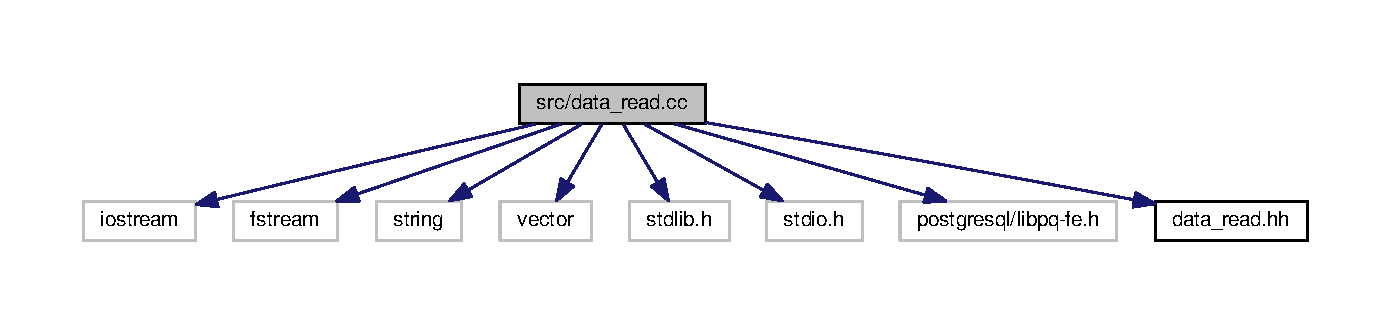
\includegraphics[width=350pt]{data__read_8cc__incl}
\end{center}
\end{figure}

\hypertarget{gold__decon_8cc}{}\section{src/gold\+\_\+decon.cc File Reference}
\label{gold__decon_8cc}\index{src/gold\+\_\+decon.\+cc@{src/gold\+\_\+decon.\+cc}}
{\ttfamily \#include $<$string$>$}\newline
{\ttfamily \#include $<$iostream$>$}\newline
{\ttfamily \#include $<$cmath$>$}\newline
{\ttfamily \#include $<$vector$>$}\newline
{\ttfamily \#include $<$algorithm$>$}\newline
{\ttfamily \#include \char`\"{}gold\+\_\+decon.\+hh\char`\"{}}\newline
Include dependency graph for gold\+\_\+decon.\+cc\+:
\nopagebreak
\begin{figure}[H]
\begin{center}
\leavevmode
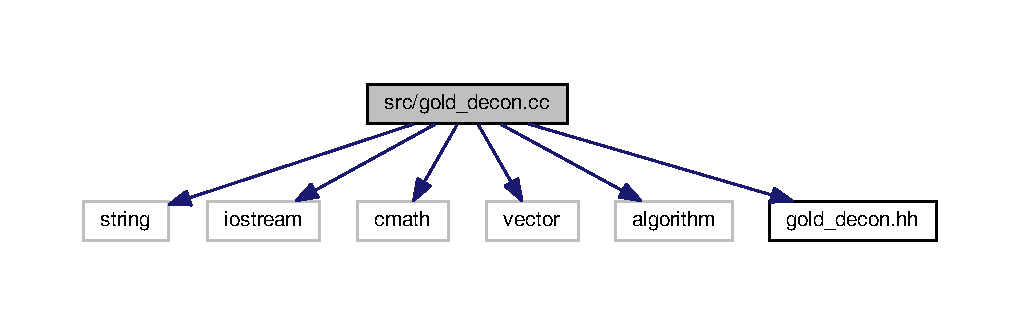
\includegraphics[width=350pt]{gold__decon_8cc__incl}
\end{center}
\end{figure}

\hypertarget{histo_8cc}{}\section{src/histo.cc File Reference}
\label{histo_8cc}\index{src/histo.\+cc@{src/histo.\+cc}}
{\ttfamily \#include $<$string$>$}\newline
{\ttfamily \#include $<$iostream$>$}\newline
{\ttfamily \#include $<$vector$>$}\newline
{\ttfamily \#include \char`\"{}histo.\+hh\char`\"{}}\newline
Include dependency graph for histo.\+cc\+:
\nopagebreak
\begin{figure}[H]
\begin{center}
\leavevmode
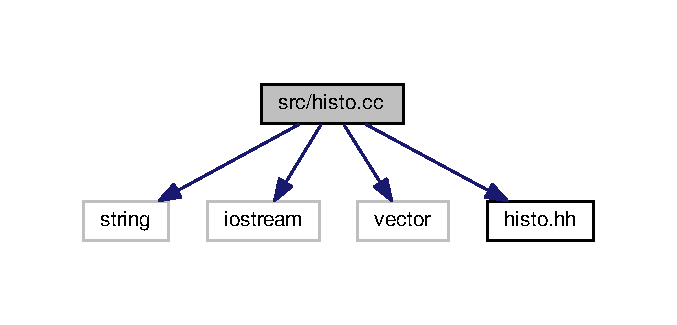
\includegraphics[width=325pt]{histo_8cc__incl}
\end{center}
\end{figure}

\hypertarget{resp__read_8cc}{}\section{src/resp\+\_\+read.cc File Reference}
\label{resp__read_8cc}\index{src/resp\+\_\+read.\+cc@{src/resp\+\_\+read.\+cc}}
{\ttfamily \#include $<$iostream$>$}\newline
{\ttfamily \#include $<$iomanip$>$}\newline
{\ttfamily \#include $<$fstream$>$}\newline
{\ttfamily \#include $<$string$>$}\newline
{\ttfamily \#include $<$vector$>$}\newline
{\ttfamily \#include $<$cmath$>$}\newline
{\ttfamily \#include \char`\"{}resp\+\_\+read.\+hh\char`\"{}}\newline
Include dependency graph for resp\+\_\+read.\+cc\+:
\nopagebreak
\begin{figure}[H]
\begin{center}
\leavevmode
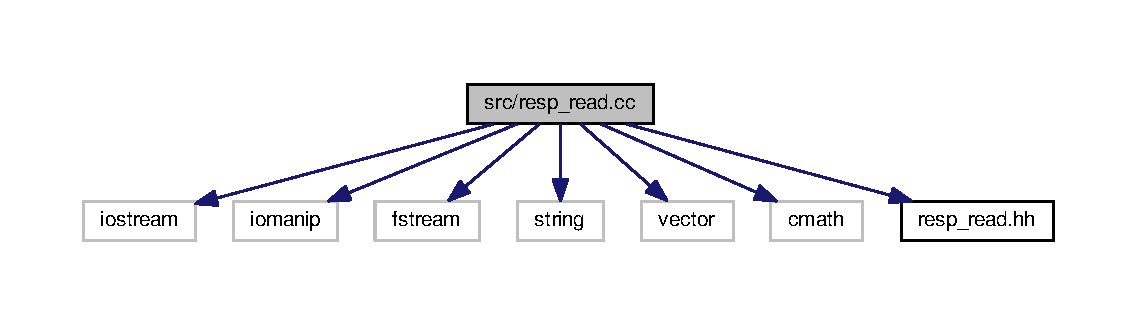
\includegraphics[width=350pt]{resp__read_8cc__incl}
\end{center}
\end{figure}

\hypertarget{sim__source_8cc}{}\section{src/sim\+\_\+source.cc File Reference}
\label{sim__source_8cc}\index{src/sim\+\_\+source.\+cc@{src/sim\+\_\+source.\+cc}}
{\ttfamily \#include $<$string$>$}\newline
{\ttfamily \#include $<$iostream$>$}\newline
{\ttfamily \#include $<$fstream$>$}\newline
{\ttfamily \#include $<$vector$>$}\newline
{\ttfamily \#include $<$cmath$>$}\newline
{\ttfamily \#include $<$stdlib.\+h$>$}\newline
{\ttfamily \#include $<$stdio.\+h$>$}\newline
{\ttfamily \#include \char`\"{}sim\+\_\+source.\+hh\char`\"{}}\newline
Include dependency graph for sim\+\_\+source.\+cc\+:
\nopagebreak
\begin{figure}[H]
\begin{center}
\leavevmode
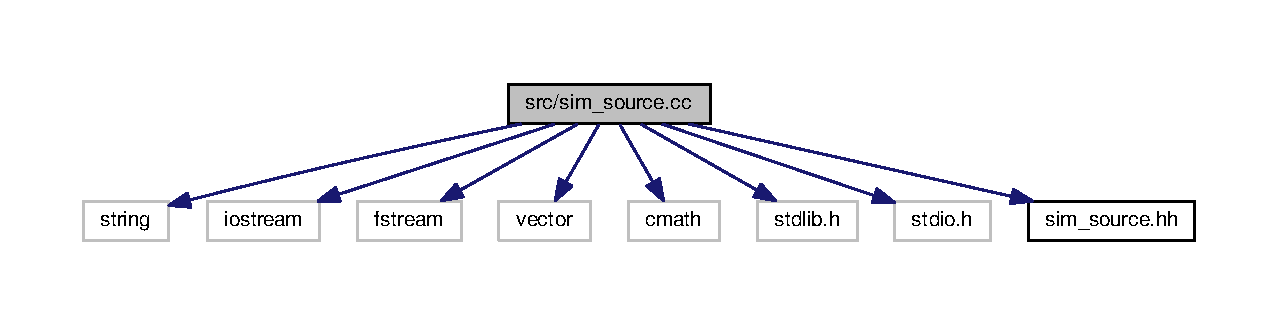
\includegraphics[width=350pt]{sim__source_8cc__incl}
\end{center}
\end{figure}

\hypertarget{spatial__decon_8cc}{}\section{src/spatial\+\_\+decon.cc File Reference}
\label{spatial__decon_8cc}\index{src/spatial\+\_\+decon.\+cc@{src/spatial\+\_\+decon.\+cc}}
{\ttfamily \#include $<$string$>$}\newline
{\ttfamily \#include $<$iostream$>$}\newline
{\ttfamily \#include $<$cmath$>$}\newline
{\ttfamily \#include $<$cstdlib$>$}\newline
{\ttfamily \#include $<$vector$>$}\newline
{\ttfamily \#include $<$ctime$>$}\newline
{\ttfamily \#include \char`\"{}spatial\+\_\+decon.\+hh\char`\"{}}\newline
Include dependency graph for spatial\+\_\+decon.\+cc\+:
\nopagebreak
\begin{figure}[H]
\begin{center}
\leavevmode
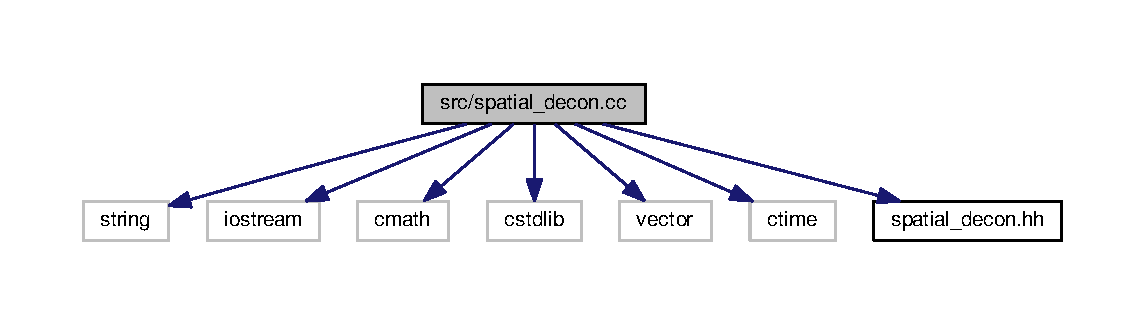
\includegraphics[width=350pt]{spatial__decon_8cc__incl}
\end{center}
\end{figure}

\hypertarget{data__read__test_8cc}{}\section{tests/data\+\_\+read\+\_\+test.cc File Reference}
\label{data__read__test_8cc}\index{tests/data\+\_\+read\+\_\+test.\+cc@{tests/data\+\_\+read\+\_\+test.\+cc}}
{\ttfamily \#include $<$iostream$>$}\newline
{\ttfamily \#include $<$string$>$}\newline
{\ttfamily \#include $<$vector$>$}\newline
{\ttfamily \#include $<$stdio.\+h$>$}\newline
{\ttfamily \#include $<$stdlib.\+h$>$}\newline
{\ttfamily \#include $<$postgresql/libpq-\/fe.\+h$>$}\newline
Include dependency graph for data\+\_\+read\+\_\+test.\+cc\+:
\nopagebreak
\begin{figure}[H]
\begin{center}
\leavevmode
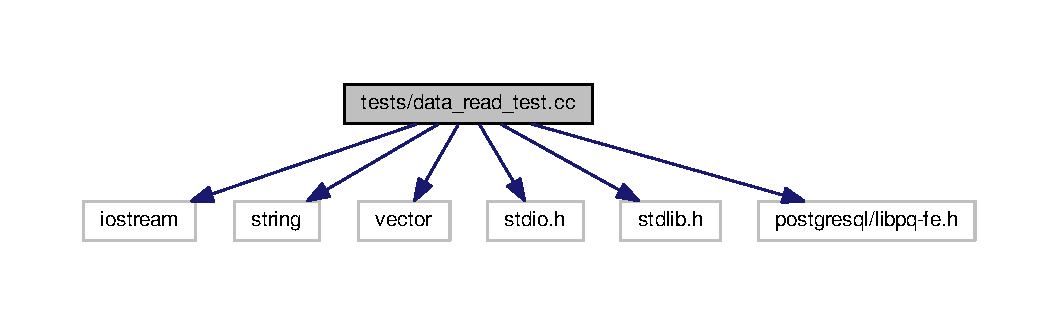
\includegraphics[width=350pt]{data__read__test_8cc__incl}
\end{center}
\end{figure}
\subsection*{Functions}
\begin{DoxyCompactItemize}
\item 
int \mbox{\hyperlink{data__read__test_8cc_ae66f6b31b5ad750f1fe042a706a4e3d4}{main}} ()
\end{DoxyCompactItemize}


\subsection{Function Documentation}
\mbox{\Hypertarget{data__read__test_8cc_ae66f6b31b5ad750f1fe042a706a4e3d4}\label{data__read__test_8cc_ae66f6b31b5ad750f1fe042a706a4e3d4}} 
\index{data\+\_\+read\+\_\+test.\+cc@{data\+\_\+read\+\_\+test.\+cc}!main@{main}}
\index{main@{main}!data\+\_\+read\+\_\+test.\+cc@{data\+\_\+read\+\_\+test.\+cc}}
\subsubsection{\texorpdfstring{main()}{main()}}
{\footnotesize\ttfamily int main (\begin{DoxyParamCaption}{ }\end{DoxyParamCaption})}


\hypertarget{sim__source__test_8cc}{}\section{tests/sim\+\_\+source\+\_\+test.cc File Reference}
\label{sim__source__test_8cc}\index{tests/sim\+\_\+source\+\_\+test.\+cc@{tests/sim\+\_\+source\+\_\+test.\+cc}}
{\ttfamily \#include $<$string$>$}\newline
{\ttfamily \#include $<$iostream$>$}\newline
{\ttfamily \#include $<$fstream$>$}\newline
{\ttfamily \#include $<$vector$>$}\newline
{\ttfamily \#include $<$cmath$>$}\newline
{\ttfamily \#include $<$stdlib.\+h$>$}\newline
{\ttfamily \#include $<$stdio.\+h$>$}\newline
{\ttfamily \#include $<$postgresql/libpq-\/fe.\+h$>$}\newline
{\ttfamily \#include \char`\"{}sim\+\_\+source.\+hh\char`\"{}}\newline
{\ttfamily \#include \char`\"{}data\+\_\+read.\+hh\char`\"{}}\newline
Include dependency graph for sim\+\_\+source\+\_\+test.\+cc\+:
\nopagebreak
\begin{figure}[H]
\begin{center}
\leavevmode
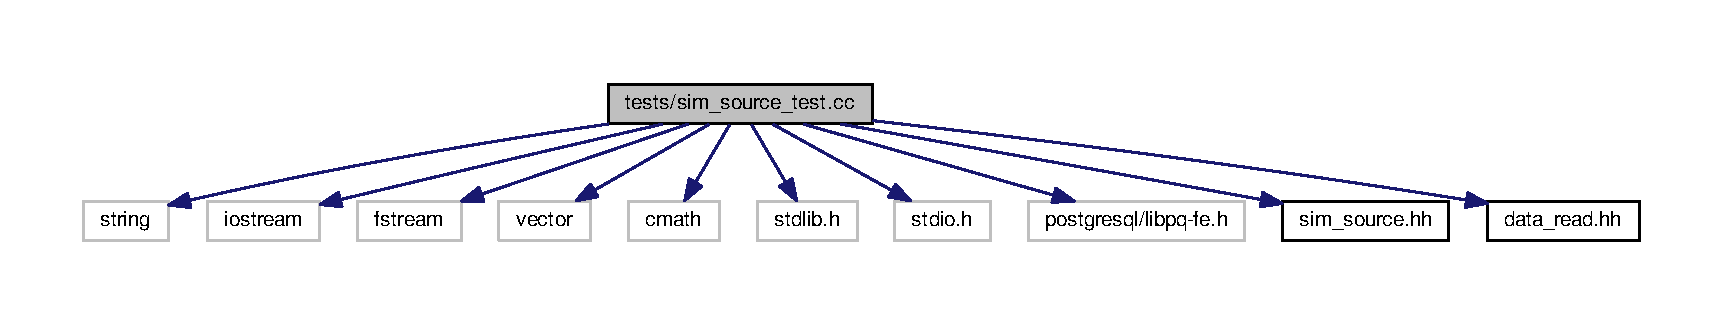
\includegraphics[width=350pt]{sim__source__test_8cc__incl}
\end{center}
\end{figure}

\hypertarget{source__read_8cc}{}\section{tests/source\+\_\+read.cc File Reference}
\label{source__read_8cc}\index{tests/source\+\_\+read.\+cc@{tests/source\+\_\+read.\+cc}}
{\ttfamily \#include $<$string$>$}\newline
{\ttfamily \#include $<$iostream$>$}\newline
{\ttfamily \#include $<$iomanip$>$}\newline
{\ttfamily \#include $<$ifstream$>$}\newline
{\ttfamily \#include $<$vector$>$}\newline
Include dependency graph for source\+\_\+read.\+cc\+:
\nopagebreak
\begin{figure}[H]
\begin{center}
\leavevmode
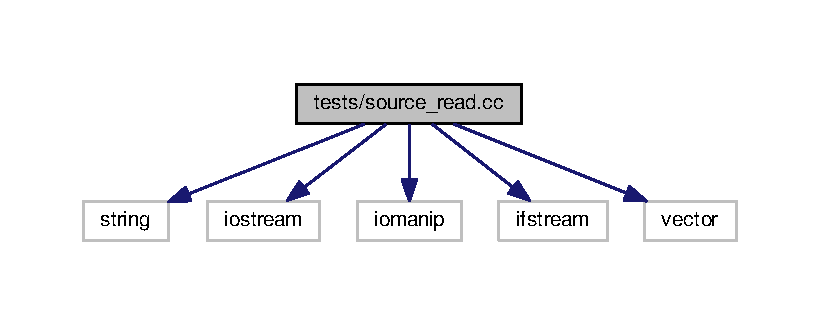
\includegraphics[width=350pt]{source__read_8cc__incl}
\end{center}
\end{figure}
\subsection*{Functions}
\begin{DoxyCompactItemize}
\item 
\mbox{\hyperlink{source__read_8cc_a630fd41d2c27aa9f32f5ed6c53ad76aa}{in\+File}} \mbox{\hyperlink{source__read_8cc_a16bc1a7a552474498051ef292208441b}{open}} (\char`\"{}source\+\_\+sim.\+txt\char`\"{})
\item 
\mbox{\hyperlink{source__read_8cc_ab6f2c6b89d54f1a92e0a2d3d6506ad66}{if}} (!\mbox{\hyperlink{source__read_8cc_a630fd41d2c27aa9f32f5ed6c53ad76aa}{in\+File}})
\item 
\mbox{\hyperlink{source__read_8cc_a816e149c6568a71e8b4e60e91677df90}{for}} (int a=0;a$<$ \mbox{\hyperlink{source__read_8cc_a0c11e7e528273d016d9f0e97efe8355b}{count}};a++)
\end{DoxyCompactItemize}
\subsection*{Variables}
\begin{DoxyCompactItemize}
\item 
int \mbox{\hyperlink{source__read_8cc_a6150e0515f7202e2fb518f7206ed97dc}{x}}
\item 
ifstream \mbox{\hyperlink{source__read_8cc_a630fd41d2c27aa9f32f5ed6c53ad76aa}{in\+File}}
\item 
int \mbox{\hyperlink{source__read_8cc_a0c11e7e528273d016d9f0e97efe8355b}{count}}
\item 
int \mbox{\hyperlink{source__read_8cc_a9b2b6fda4c98c1de0b9123c78a72a95d}{numbers}} \mbox{[}\mbox{\hyperlink{source__read_8cc_a0c11e7e528273d016d9f0e97efe8355b}{count}}\mbox{]}
\end{DoxyCompactItemize}


\subsection{Function Documentation}
\mbox{\Hypertarget{source__read_8cc_a816e149c6568a71e8b4e60e91677df90}\label{source__read_8cc_a816e149c6568a71e8b4e60e91677df90}} 
\index{source\+\_\+read.\+cc@{source\+\_\+read.\+cc}!for@{for}}
\index{for@{for}!source\+\_\+read.\+cc@{source\+\_\+read.\+cc}}
\subsubsection{\texorpdfstring{for()}{for()}}
{\footnotesize\ttfamily for (\begin{DoxyParamCaption}{ }\end{DoxyParamCaption})}

\mbox{\Hypertarget{source__read_8cc_ab6f2c6b89d54f1a92e0a2d3d6506ad66}\label{source__read_8cc_ab6f2c6b89d54f1a92e0a2d3d6506ad66}} 
\index{source\+\_\+read.\+cc@{source\+\_\+read.\+cc}!if@{if}}
\index{if@{if}!source\+\_\+read.\+cc@{source\+\_\+read.\+cc}}
\subsubsection{\texorpdfstring{if()}{if()}}
{\footnotesize\ttfamily if (\begin{DoxyParamCaption}\item[{!}]{in\+File }\end{DoxyParamCaption})}

\mbox{\Hypertarget{source__read_8cc_a16bc1a7a552474498051ef292208441b}\label{source__read_8cc_a16bc1a7a552474498051ef292208441b}} 
\index{source\+\_\+read.\+cc@{source\+\_\+read.\+cc}!open@{open}}
\index{open@{open}!source\+\_\+read.\+cc@{source\+\_\+read.\+cc}}
\subsubsection{\texorpdfstring{open()}{open()}}
{\footnotesize\ttfamily \mbox{\hyperlink{source__read_8cc_a630fd41d2c27aa9f32f5ed6c53ad76aa}{in\+File}} open (\begin{DoxyParamCaption}\item[{\char`\"{}source\+\_\+sim.\+txt\char`\"{}}]{ }\end{DoxyParamCaption})}



\subsection{Variable Documentation}
\mbox{\Hypertarget{source__read_8cc_a0c11e7e528273d016d9f0e97efe8355b}\label{source__read_8cc_a0c11e7e528273d016d9f0e97efe8355b}} 
\index{source\+\_\+read.\+cc@{source\+\_\+read.\+cc}!count@{count}}
\index{count@{count}!source\+\_\+read.\+cc@{source\+\_\+read.\+cc}}
\subsubsection{\texorpdfstring{count}{count}}
{\footnotesize\ttfamily \mbox{\hyperlink{source__read_8cc_a630fd41d2c27aa9f32f5ed6c53ad76aa}{in\+File}} count}

\mbox{\Hypertarget{source__read_8cc_a630fd41d2c27aa9f32f5ed6c53ad76aa}\label{source__read_8cc_a630fd41d2c27aa9f32f5ed6c53ad76aa}} 
\index{source\+\_\+read.\+cc@{source\+\_\+read.\+cc}!in\+File@{in\+File}}
\index{in\+File@{in\+File}!source\+\_\+read.\+cc@{source\+\_\+read.\+cc}}
\subsubsection{\texorpdfstring{in\+File}{inFile}}
{\footnotesize\ttfamily ifstream in\+File}

\mbox{\Hypertarget{source__read_8cc_a9b2b6fda4c98c1de0b9123c78a72a95d}\label{source__read_8cc_a9b2b6fda4c98c1de0b9123c78a72a95d}} 
\index{source\+\_\+read.\+cc@{source\+\_\+read.\+cc}!numbers@{numbers}}
\index{numbers@{numbers}!source\+\_\+read.\+cc@{source\+\_\+read.\+cc}}
\subsubsection{\texorpdfstring{numbers}{numbers}}
{\footnotesize\ttfamily int numbers\mbox{[}\mbox{\hyperlink{source__read_8cc_a0c11e7e528273d016d9f0e97efe8355b}{count}}\mbox{]}}

\mbox{\Hypertarget{source__read_8cc_a6150e0515f7202e2fb518f7206ed97dc}\label{source__read_8cc_a6150e0515f7202e2fb518f7206ed97dc}} 
\index{source\+\_\+read.\+cc@{source\+\_\+read.\+cc}!x@{x}}
\index{x@{x}!source\+\_\+read.\+cc@{source\+\_\+read.\+cc}}
\subsubsection{\texorpdfstring{x}{x}}
{\footnotesize\ttfamily int x}


\hypertarget{unfold_8cc}{}\section{tests/unfold.cc File Reference}
\label{unfold_8cc}\index{tests/unfold.\+cc@{tests/unfold.\+cc}}
{\ttfamily \#include $<$T\+H2.\+h$>$}\newline
{\ttfamily \#include $<$T\+File.\+h$>$}\newline
{\ttfamily \#include $<$T\+System.\+h$>$}\newline
{\ttfamily \#include $<$T\+Math.\+h$>$}\newline
{\ttfamily \#include $<$T\+Tree.\+h$>$}\newline
{\ttfamily \#include $<$T\+String.\+h$>$}\newline
{\ttfamily \#include $<$T\+Ntuple.\+h$>$}\newline
{\ttfamily \#include $<$iostream$>$}\newline
{\ttfamily \#include $<$T\+Class.\+h$>$}\newline
{\ttfamily \#include $<$T\+Application.\+h$>$}\newline
{\ttfamily \#include $<$sys/time.\+h$>$}\newline
{\ttfamily \#include $<$ctime$>$}\newline
Include dependency graph for unfold.\+cc\+:
\nopagebreak
\begin{figure}[H]
\begin{center}
\leavevmode
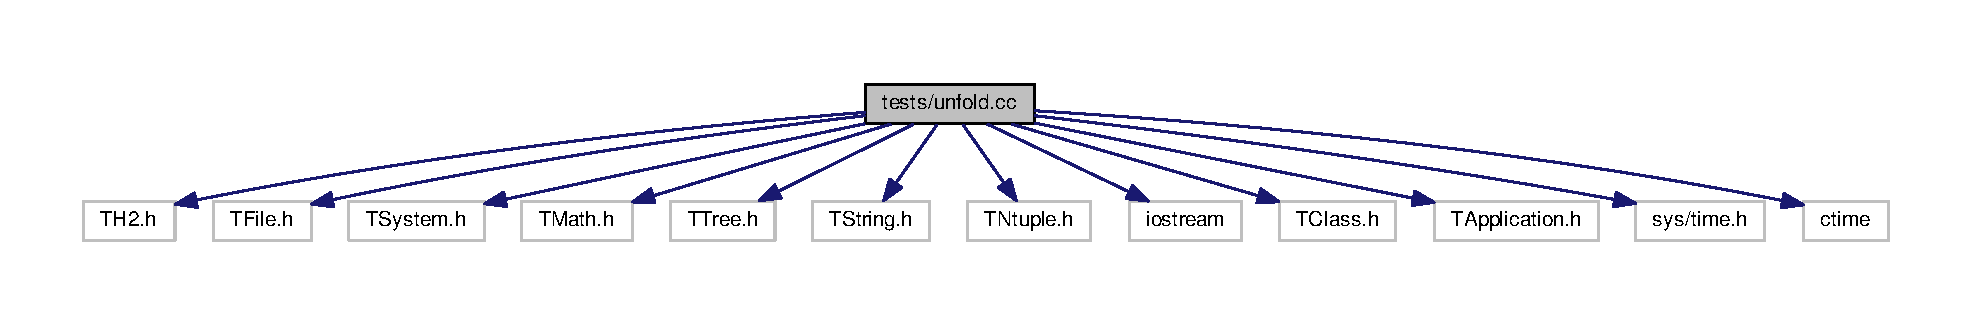
\includegraphics[width=350pt]{unfold_8cc__incl}
\end{center}
\end{figure}
\subsection*{Typedefs}
\begin{DoxyCompactItemize}
\item 
typedef unsigned long long \mbox{\hyperlink{unfold_8cc_a29217083807c6b153656eda1a04f306d}{timestamp\+\_\+t}}
\end{DoxyCompactItemize}
\subsection*{Functions}
\begin{DoxyCompactItemize}
\item 
void \mbox{\hyperlink{unfold_8cc_a629708a3e6e3e31be73df380974987a9}{normalize}} (float $\ast$)
\item 
void \mbox{\hyperlink{unfold_8cc_abc893c4d407fd5b8bc451ce5c9fa290c}{multiply}} (float $\ast$$\ast$, float $\ast$)
\item 
void \mbox{\hyperlink{unfold_8cc_a711c23f90c830e749c9c849e6282647d}{do\+Refold}} (float $\ast$, float $\ast$$\ast$)
\item 
double \mbox{\hyperlink{unfold_8cc_a2df7244a9a191cce709c4e70e2ed3e9f}{calculate\+Residual}} (float $\ast$, float $\ast$)
\item 
const char $\ast$ \mbox{\hyperlink{unfold_8cc_a595837c698e2cdaed6f87491ef06f4aa}{do\+Unfold}} (float $\ast$, float $\ast$$\ast$, int, int, int, int, double)
\item 
int \mbox{\hyperlink{unfold_8cc_a3c04138a5bfe5d72780bb7e82a18e627}{main}} (int argc, char $\ast$$\ast$argv)
\end{DoxyCompactItemize}


\subsection{Typedef Documentation}
\mbox{\Hypertarget{unfold_8cc_a29217083807c6b153656eda1a04f306d}\label{unfold_8cc_a29217083807c6b153656eda1a04f306d}} 
\index{unfold.\+cc@{unfold.\+cc}!timestamp\+\_\+t@{timestamp\+\_\+t}}
\index{timestamp\+\_\+t@{timestamp\+\_\+t}!unfold.\+cc@{unfold.\+cc}}
\subsubsection{\texorpdfstring{timestamp\+\_\+t}{timestamp\_t}}
{\footnotesize\ttfamily typedef unsigned long long \mbox{\hyperlink{unfold_8cc_a29217083807c6b153656eda1a04f306d}{timestamp\+\_\+t}}}



\subsection{Function Documentation}
\mbox{\Hypertarget{unfold_8cc_a2df7244a9a191cce709c4e70e2ed3e9f}\label{unfold_8cc_a2df7244a9a191cce709c4e70e2ed3e9f}} 
\index{unfold.\+cc@{unfold.\+cc}!calculate\+Residual@{calculate\+Residual}}
\index{calculate\+Residual@{calculate\+Residual}!unfold.\+cc@{unfold.\+cc}}
\subsubsection{\texorpdfstring{calculate\+Residual()}{calculateResidual()}}
{\footnotesize\ttfamily double calculate\+Residual (\begin{DoxyParamCaption}\item[{float $\ast$}]{source1,  }\item[{float $\ast$}]{source2 }\end{DoxyParamCaption})}

\mbox{\Hypertarget{unfold_8cc_a711c23f90c830e749c9c849e6282647d}\label{unfold_8cc_a711c23f90c830e749c9c849e6282647d}} 
\index{unfold.\+cc@{unfold.\+cc}!do\+Refold@{do\+Refold}}
\index{do\+Refold@{do\+Refold}!unfold.\+cc@{unfold.\+cc}}
\subsubsection{\texorpdfstring{do\+Refold()}{doRefold()}}
{\footnotesize\ttfamily void do\+Refold (\begin{DoxyParamCaption}\item[{float $\ast$}]{source\+In,  }\item[{float $\ast$$\ast$}]{RF }\end{DoxyParamCaption})}

\mbox{\Hypertarget{unfold_8cc_a595837c698e2cdaed6f87491ef06f4aa}\label{unfold_8cc_a595837c698e2cdaed6f87491ef06f4aa}} 
\index{unfold.\+cc@{unfold.\+cc}!do\+Unfold@{do\+Unfold}}
\index{do\+Unfold@{do\+Unfold}!unfold.\+cc@{unfold.\+cc}}
\subsubsection{\texorpdfstring{do\+Unfold()}{doUnfold()}}
{\footnotesize\ttfamily const char $\ast$ do\+Unfold (\begin{DoxyParamCaption}\item[{float $\ast$}]{source,  }\item[{float $\ast$$\ast$}]{resp\+Matrix,  }\item[{int}]{ssizex,  }\item[{int}]{ssizey,  }\item[{int}]{number\+Iterations,  }\item[{int}]{number\+Repetitions,  }\item[{double}]{boost }\end{DoxyParamCaption})}

\mbox{\Hypertarget{unfold_8cc_a3c04138a5bfe5d72780bb7e82a18e627}\label{unfold_8cc_a3c04138a5bfe5d72780bb7e82a18e627}} 
\index{unfold.\+cc@{unfold.\+cc}!main@{main}}
\index{main@{main}!unfold.\+cc@{unfold.\+cc}}
\subsubsection{\texorpdfstring{main()}{main()}}
{\footnotesize\ttfamily int main (\begin{DoxyParamCaption}\item[{int}]{argc,  }\item[{char $\ast$$\ast$}]{argv }\end{DoxyParamCaption})}

\mbox{\Hypertarget{unfold_8cc_abc893c4d407fd5b8bc451ce5c9fa290c}\label{unfold_8cc_abc893c4d407fd5b8bc451ce5c9fa290c}} 
\index{unfold.\+cc@{unfold.\+cc}!multiply@{multiply}}
\index{multiply@{multiply}!unfold.\+cc@{unfold.\+cc}}
\subsubsection{\texorpdfstring{multiply()}{multiply()}}
{\footnotesize\ttfamily void multiply (\begin{DoxyParamCaption}\item[{float $\ast$$\ast$}]{RF,  }\item[{float $\ast$}]{source }\end{DoxyParamCaption})}

\mbox{\Hypertarget{unfold_8cc_a629708a3e6e3e31be73df380974987a9}\label{unfold_8cc_a629708a3e6e3e31be73df380974987a9}} 
\index{unfold.\+cc@{unfold.\+cc}!normalize@{normalize}}
\index{normalize@{normalize}!unfold.\+cc@{unfold.\+cc}}
\subsubsection{\texorpdfstring{normalize()}{normalize()}}
{\footnotesize\ttfamily void normalize (\begin{DoxyParamCaption}\item[{float $\ast$}]{spectrum }\end{DoxyParamCaption})}


%--- End generated contents ---

% Index
\backmatter
\newpage
\phantomsection
\clearemptydoublepage
\addcontentsline{toc}{chapter}{Index}
\printindex

\end{document}
